\documentclass[fr]{../../../eplsummary}

\usepackage{../../../eplchem}
\usepackage[SIunits]{../../../eplunits}

\usepackage{multirow}
\usepackage{color}
\usepackage{chemfig}
\usepackage{tikz}
\usepackage{pgfplots}
\usepackage{pgffor}
\usepackage{qtree}

\renewcommand{\textbf}[1]{\begingroup\bfseries\mathversion{bold}#1\endgroup}

\newcommand\sorb{\mathrm{s}}
\newcommand\porb{\mathrm{p}}
\newcommand\dorb{\mathrm{d}}
\newcommand\forb{\mathrm{f}}
\newcommand\gorb{\mathrm{g}}
\newcommand\gaz{\ensuremath{_{(g)}}}
\newcommand\solid{\ensuremath{_{(s)}}}
\newcommand\liquid{\ensuremath{_{(l)}}}
\newcommand\debye{\mathrm{D}}
\newcommand\calo{\mathrm{cal}}
\newcommand\atm{\mathrm{atm}}
\newcommand\ccal{\ensuremath{C_\mathrm{cal}}}
\newcommand\qrev{\ensuremath{q_{\mathrm{rév}}}}
\newcommand\kc{\ensuremath{K_{\mathrm{c}}}}
\newcommand\kp{\ensuremath{K_{\mathrm{p}}}}
\newcommand\keq{\ensuremath{K_{\mathrm{éq}}}}
\newcommand\pkb{\mathrm{p}\ensuremath{K_b}}
\newcommand\pka{\mathrm{p}\ensuremath{K_a}}

\hypertitle{Chimie}{2}{FSAB}{1301}
{Beno\^it Legat\and Lucas Nyssens\and Laurent Opsomer\and Antoine Paris}
{Sophie Demoustier, Alain Jonas et Bernard Nysten}

\paragraph{Remarque préliminaire}
Dans certaines formules,
des variables seront utilisées sans expliciter leur signification.
C'est du au fait qu'elle sont très couramment utilisée
ce qui rend leur signification implicite.
Elles sont tout de même listée à l'Annexe~\ref{ann:nota}.

\part{Notions de base}

\paragraph{Propriétés de la matière}
\begin{itemize}
  \item Propriétés \textbf{extensives}: Dépendent de la quantité de matière (Ex: Masse, énergie,...).
  \item Propriétés \textbf{intensives}: Ne dépendent pas de la quantité de matière (Ex: Température, pression,...).
\end{itemize}

\paragraph{A. Lavoisier}
\begin{enumerate}
  \item Loi de conservation de la masse: ``Dans un conteneur étanche, ni création, ni perte de matière''.
  \item Loi des compositions définies: ``Dans un composé pur, les éléments sont toujours présents dans des proportions définies''.
\end{enumerate}

\paragraph{Chaleur de réaction:}
\'Energie de réaction: énergie absorbée par le système (par convention)
$$\Delta E = E_{\textrm{produits}}-E_{\textrm{réactifs}}$$

Si réaction endothermique: absorption d'énergie $\Rightarrow \Delta E > 0$

Si réaction exothermique: dégagement d'énergie $\Rightarrow  \Delta E < 0$

\part{Atomistique}

%\subsection{\'Electrons de coeur}
%Les électrons de coeur sont tous les électrons sauf les électrons de valences.

%\paragraph{Exemple}
%$\ce{Zn}$ de composition $[\ce{Ar}]3\dorb^{10}4\sorb^{2}$
%a 28 électrons de coeur car $\ce{Ar}$ a 18 électrons
%et la derniére couche est $n=4$,
%donc $3\dorb^{10}$ n'y est pas et peut être compté.
%On peut aussi dire qu'il en a 18 en prenant une valence de 12.

\paragraph{Nombres atomiques et de masse}

\emph{$^{A}_{Z}X$}
\begin{itemize}
  \item $Z$: nombre atomique = nombre de protons dans le noyau = nombre d'électrons
  \item $A$: nombre de masse = nombre de protons et de neutrons dans le noyau (car masse $e^{-}$ négligeable)
  \item \# neutrons = $A-Z$
  \item Isotopes: même nombre de protons, nombre de neutrons différent.
\end{itemize}

\section{Rayonnement électromagnétique}

La lumière, les ondes radios,...
sont des formes de rayonnements électromagnétiques constitués d'un champ électrique oscillant et d'un champ magnétique oscillant $\Rightarrow$ transportent de l'énergie.

Caractéristiques:
\begin{itemize}
  \item Longueur d'onde $\lambda$ (\meter)
  \item Fréquence $\nu$ (\hertz)
  \item Vitesse (de la lumière) $c$ (\meter\per\second)
\end{itemize}

On sait que
\begin{equation}
  \label{eq:clambdanu}
  c = \lambda \nu
\end{equation}

Si le rayonnement est dans le vide
\[ c = c_0 \]

Un rayonnement électromagnétique ne peut transmettre de l'énergie que par {\it quanta},
qui est l'énergie transmise par un photon et qui vaut
\begin{equation}
  \label{eq:Ehnu}
  E = h\nu
\end{equation}

L'énergie émise par un atome dont un électron passe d'une couche à une distance $n_i$ à un couche à une distance $n_f$ vaut
\[ \Delta E = h\nu = \frac{hc}{\lambda} = R_y \left( \frac{1}{n_f^2} - \frac{1}{n_i^2} \right) \]
où $R_y = hc R_\infty = \numprint[\joule]{2,178e-18}$ est la constante de Rydberg.

Si un électron se déplace d'une couche plus éloignée à une couche moins éloignée,
un photon est émis par l'atome et si un photon apporte son énergie à un atome,
un électron va se déplacer d'une couche moins éloignée à une couche plus éloignée.

\subsection{Longueur d'onde de Broglie}
Toute particule physique dotée d'une quantité de mouvement a une longueur
d'onde, nommée longueur d'onde de Broglie, qui est donnée par
\[ \lambda = \frac{h}{p} = \frac{h}{mv} \]

Il est amusant d'observer qu'en utilisant les formules vues plus haut
et la longueur d'onde de Broglie dans le cas d'un rayonnement électromagnétique,
c'est à dire que $v = c$, on trouve
\[ E \stackrel{\eqref{eq:Ehnu}}{=} h\nu = mc\lambda\nu \stackrel{\eqref{eq:clambdanu}}{=} mc^2 \]

Les électrons (et la matière en général) ont à la fois un caractère ondulatoire et un caractère corpusculaire.


\section{Fonction d'onde}

Dualité onde-particule $\Rightarrow$ les électrons ne tournent pas autour du noyau selon une trajectoire définie.

$\Rightarrow$ Fonction d'onde $\psi$ (solutions équation de Schrödinger)\\

Max Born: $\psi^2 = $ densité de probabilité de présence de la particule (probabilité de présence/volume).

Les \textbf{orbitales atomiques} sont les fonctions d'onde des électrons dans les atomes.

\section{Nombres quantiques}

Un électron dans un atome voyage toujours sur une orbitale.
Deux électrons ne peuvent pas être tous les deux
sur la même orbitale dans un même sens.
Les orbitales peuvent être décrites par 3 paramètres.

\subsection{Le nombre quantique principal}
L'électron se déplace dans son orbite le long d'une sinusoïde,
$n$ détermine le nombre de période qu'il fait par tour.
Comme $n$ est un nombre naturel,
il faut que la circonférence de l'orbite soit un multiple de $\lambda$.
C'est à dire
\[ n\lambda = 2\pi r \]

Par la longueur d'onde de Broglie
\[ n \frac{h}{2\pi} = m v r \]

$n$ détermine donc aussi le rayon de l'orbitale et son énergie.
On voit que $n$ est proportionnel au rayon de l'orbitale.
$n$ peut prendre les valeurs $1, 2, \ldots$

$n$ détermine la couche de l'orbitale.
%La valeur de $n$ peut aussi être représenté par la période correspondante
% NOT SURE
%\begin{center}
%\begin{tabular}{c|ccccc}
%	$n$ & 1 & 2 & 3 & 4 & \multirow{2}{*}{$\cdots$}\\
%	\cline{1-5}
%	Période & K & L & M & N
%\end{tabular}
%\end{center}

\subsection{Le nombre quantique secondaire}
$l$ détermine la forme de l'orbitale.
Il y a exactement $n$ formes possible pour une orbitale de nombre quantique $n$.

{\bf La numérotation se fait}, comme en informatique, {\bf à partir de $0$}.
Pour une orbitale de nombre quantique $n$, $l$ peut prendre les valeurs $0, 1, \ldots, n-1$

$l$ détermine la sous-couche de l'orbitale.

La valeur de $l$ peut aussi être représenté par une lettre minuscule

\begin{center}
  \begin{tabular}{c|cccccc}
    $l$ & 0 & 1 & 2 & 3 & 4 & \multirow{2}{*}{$\cdots$}\\
    \cline{1-6}
    Lettre & $\sorb$ & $\porb$ & $\dorb$ & $\forb$ & $\gorb$\\
    Origine & {\bf s}harp & {\bf p}rincipal & {\bf d}iffuse & {\bf f}ondamental
  \end{tabular}
\end{center}

\subsection{Le nombre quantique magnétique}
$m_l$ détermine l'orientation relative de l'orbitale par rapport aux autres orbitales de sa sous-couche.
Il y a exactement $2l + 1$ orientation possible pour une orbitale de nombre quantique $l$.
Pour une orbitale de nombre quantique $l$, $m_l$ peut prendre les valeurs $-l, \ldots, -1,  0, 1, \ldots, l$

\subsection{Le nombre quantique de spin}
$m_s$ détermine le sens dans lequel l'électron se déplace.
$m_s$ peut prendre les valeurs $-\frac{1}{2}$ et $\frac{1}{2}$.

La valeur de $m_s$ peut aussi être représenté par l'orientation du moment magnétique de l'électron dans l'orbitale correspondante
\begin{center}
  \begin{tabular}{c|cc}
    $m_s$ & $-\frac{1}{2}$ & $\frac{1}{2}$\\
    \hline
    Moment magnétique & down & up
  \end{tabular}
\end{center}

$m_s$ ne décrit pas l'orbitale mais l'électron dans celle ci,
c'est pourquoi on dit qu'une orbitale est définie par 3 nombres quantiques et non 4.

% E ^
%  n v
%  r v
%  Z ^
%  Ecrantage v
% s > p > d > f

\section{Structure électronique de l'hydrogène}
\begin{itemize}
  \item \'Etat fondamental: l'$e^-$ occupe une orbitale 1s
  \item Si l'$e^-$ acquiert assez d'énergie,
    il peut atteindre d'autres couches:
    $n=2$ (2s ou une des trois sous-couches 2p),
    $n=3,4,\ldots$
    et s'il acquiert suffisamment d'énergie $\rightarrow$ quitte l'atome.
\end{itemize}

Les atomes hydrogénoïdes ont des sous-couches dégénérées, c'est-à-dire que les orbitales associées au même nombre quantique principal ont la même énergie.
Par exemple, pour \ce{O^7+}, l'énergie associée à l'orbitale 2s est la même que celle associée à l'orbitale 2p.

On entend par atomes hydrogénoïdes, les atomes ou ions qui possèdent exactement $1$ électron (par exemple: \ce{H}, \ce{He^+}, \ce{O^7+}, ...).
On dit aussi qu'ils sont monoélectroniques.

\section{Atomes polyélectroniques}
\begin{itemize}
  \item \'Ecrantage: Chaque électron est blindé contre l’attraction complète du noyau par les couches inférieures d'électrons (répulsions interélectroniques)
    $\Rightarrow$ la charge effective $Z_{eff}$ (la charge réellement subie par les électrons) diminue et les $e^-$ sont donc moins attirés par le noyau.
  \item Effet de pénétration des $e^-$: un $e^-$ $\sorb$ de n'importe quelle couche peut se trouver près du noyau
    $\rightarrow$ il peut pénétrer à travers les couches internes.
    Un $e^-$ $\porb$ pénètre beaucoup moins (sa fonction d'onde s'annule sur le noyau) $\Rightarrow$ charge nucléaire effective inférieure à celle que subit l'$e^-$ $\sorb$.
  \item \'Energie fonction de $n$ et de $l$.
\end{itemize}
$\Rightarrow$ Ordre des énergies des orbitales: $\sorb<\porb<\dorb<\forb<...$
Pour une même couche,
il faut donc plus d'énergie pour arracher un $e^-$ de la sous-couche $\sorb$ que de la sous-couche $\porb$.

On remarquera aussi qu'un électron est repoussé par les autres électrons présents sur la même orbitale que la sienne, mais que cette répulsion est beaucoup moins importante
que celle provenant des orbitales inférieures.

\section{Remplissage des orbitales}
\begin{description}
  \item[Règle de Klechkowsky]
    Remplissage des orbitales par ordre croissant d'énergie.
  \item[Principe d'exclusion de Pauli]
    Deux électrons ne peuvent pas occuper un même état quantique dans 1 atome.
    Il y a maximum 2 $e^-$ par orbitale, un {\em up} et un {\em down}.
  \item[Règle de Hund]
    Maximisation du nombre d'$e^-$ non-appariés de spins parallèles dans un ensemble d'orbitales de même énergie.
    C'est à dire, par exemple, pour remplir l'orbitale $2\porb$,
    on commence par mettre un électron pour chaque $m_l$, tous de spin parallèle
    ({\em up} ou {\em down}, c'est relatif).
    Puis seulement, on met les 3 autres électrons s'appariant aux électrons déjà mis.
\end{description}

Exemple: le fluore: \ce{F} $1s^2 2s^2 2p^5$ ou [\ce{He}]$2s^2 2p^5$


\section{Rayon atomique}
Le rayon atomique est la moitié de la distance séparant les noyaux de 2 atomes voisins.
\begin{itemize}
  \item[$\diamond$]En général, diminution de gauche à droite dans une période :
  $\uparrow$nombre de protons $\Rightarrow$ $\uparrow$attraction dans une même couche $\Rightarrow$  $\downarrow$rayon
  \item[$\diamond$]En général, augmentation de haut en bas dans un groupe :
  $\uparrow$nombre de couches $\Rightarrow$ $\uparrow$écrantage $\Rightarrow$ $\uparrow$rayon
\end{itemize}

\section{\'Energie d'ionisation}
\label{sec:ioni}

$E_I$ = énergie absorbée pour arracher un électron de l'atome \textbf{en phase gazeuse}.
$$\ce{X(g) -> X+(g) + e-}$$

$\Delta H = E(\ce{X^+})-E(\ce{X}) = E_I$

\begin{itemize}
  \item Toujours endothermique;
  \item $E_I$ diminue globalement de haut en bas d'un groupe (quand le rayon atomique augmente).
    En effet il faut fournir moins d'énergie pour arracher un $e^-$ loin du noyau;
  \item $E_I$ augmente globalement le long d'une période à cause de l'augmentation de la charge nucléaire effective;
  \item La répulsion entre 2 $e^-$ d'une même orbitale augmente leur énergie et rend le départ d'un électron + facile que dans le cas de 2 $e^-$ non-appariés;
  \item Les électrons de valences sont arrachés en premier.
    Plus précisément,
    l'électron doit être pris dans l'orbitale au plus grand $n$,
    puis au plus grand $l$ puis commencer par les électrons appariés.
    Pour les métaux de transition,
    les $e^-$ de la sous-couche $\sorb$ de la dernière couche sont enlevés les premiers;
  \item L'ion résultant est appelé ``cation'';
  \item Rayon cationique < Rayon atomique.
\end{itemize}

\section{\'Electroaffinité}
\label{sec:electro}

$E_A$ = énergie dégagée lors de la capture d'un électron par l'atome \textbf{en phase gazeuse}.
\[ \ce{X(g) + e- -> X^-(g)} \]

$\Delta H = E(\ce{X^-})-E(\ce{X})=-E_A$

\begin{itemize}
  \item Capture du 1\up{er} $e^-$: en général exothermique;
  \item Capture du 2\up{ème} $e^-$: toujours endothermique;
  \item $E_A$ augmente globalement vers la droite du tableau périodique (si le rayon atomique diminue).
    Il y a des exeptions comme:
    pour \ce{Na},
    $E_A = \numprint[\kilo\joule\per\mole]{+53}$ alors que pour \ce{Mg},
    $E_A \leq \numprint[\kilo\joule\per\mole]{0}$;
  \item Les gaz nobles ont une $E_A$ légèrement négative (endothermique) car tout $e^-$ ajouté occupe une orbitale au-delà d'une couche pleine et loin du noyau.
    Mais comme ils sont très stables,
    $E_A \approx 0$;
  \item L'ion résultant est appelé ``anion'';
  \item Rayon anionique > Rayon atomique.
\end{itemize}

\part{Les liaisons chimiques}
\section{Liaisons intramoléculaires}
\paragraph{Remarque} Représentation de Lewis: notation des atomes avec leurs $e^-$ de valence.

\subparagraph{Exemple} L'azote:\hspace{0.7cm} \lewis{0.2.46.,N}

\subsection{Liaisons métalliques}
Pour les métaux,
l'énergie d'ionisation et l'électroaffinité sont faibles,
il y a peu d'électrons de valence et ils sont peu liés au noyau $\Rightarrow$
délocalisation des électrons (gaz d'$e^-$ libres).
Cela explique la conductivité des métaux et leur ductilité
\footnote{Propriété de certains matériaux (essentiellement les métaux)
de pouvoir être étirés et allongés sans se rompre.}.
\paragraph{Caractéristiques}
\begin{itemize}
  \item conducteurs d'électricité;
  \item déformables, plastiques;
  \item liaison \emph{forte} et \emph{isotrope} (toutes les directions).
\end{itemize}

\subsection{Liaisons ioniques}
Interaction électrostatique entre ions de charges opposées.
\paragraph{Caractéristiques}
\begin{itemize}
  \item transfert d'électrons du cation vers l'anion;
  \item rigidité et fragilité des solides ioniques;
  \item le transfert est favorisé si la configuration électronique de l'anion
    et du cation est la configuration électronique d'un gaz noble;
  \item liaison \emph{forte} et \emph{isotrope} (toutes les directions).
\end{itemize}

\paragraph{Calcul de l'énergie de liaison ionique}
\[ \ce{M + X -> M+X-} \]
\begin{center}
  \begin{tabular}{llll}
    \'Energie d'ionisation & $\ce{M -> M+ + e-}$ & $\Delta E = E_I > 0$ & endo\\
    \'Electroaffinité & $\ce{X + e- -> X-}$ & $\Delta E = E_A < 0$ & exo\\
    \'Energie de neutralisation & $\ce{M+ + X- -> M+X-}$ & $\Delta E = E_N < 0$ & exo
  \end{tabular}
\end{center}
\[ E_{\mathrm{liaison}} = E_A + E_N + E_I \]
Attention !
Pour $E_N$,
certaines tables donnent son opposé, $-E_N$.
Vérifiez bien que la plupart soient négatifs !

\paragraph{Calcul de l'énergie de neutralisation $E_N$}
\label{sec:neutral}
L'énergie de neutralisation est l'énergie à fournir pour lier deux atomes déjà ionisés.

\subparagraph{Pour les gaz}
\[ E_N = \frac{-N_A}{4\pi\epsilon_0}\times\frac{|z_1z_2|e^2}{d} \]
où $z_1$ et $z_2$ sont les valences des atomes,
$e$ la charge d'un électron et $d = r_{\mathrm{anion}} + r_{\mathrm{cation}}$ la distance entre leurs centres atomiques.
\subparagraph{Pour les solides ioniques}
Interaction entre un grand nombre d'anions et de cations.
L'alternance anion-cation rend les solides ioniques rigides et fragiles.

Distance inter-ionique: équilibre entre : l'attraction coulombienne ($-\frac{1}{d}$) et la répulsion des nuages d'électrons ($\frac{1}{d^n}$).
\[ E_N = \frac{-N_A}{4\pi\epsilon_0}\times\frac{|z_1z_2|e^2}{d} \left(1-\frac{d^*}{d}\right)A \]
où $d^* = \numprint[\pico\meter]{34,5}$,
$A$ est la constante de Madelung qui varie selon les composés et $d$ est comme pour les gaz.

\subsection{Liaison covalente}

Les électrons sont apportés par chaque atome et s'apparient $\Rightarrow$ état de moindre énergie (équilibre entre attraction $e^-$/noyau et répulsion noyau/noyau).

\paragraph{Caractéristiques}
\begin{itemize}
  \item partage d'électrons de valence;
  \item rigidité et fragilité des solides covalents;
  \item la liaison est favorisée si $E_I$ et $E_A$ sont élevées;
  \item liaison \emph{forte} et \emph{anisotrope}.
\end{itemize}
\subsubsection{Structure de Lewis}
\paragraph{Règle de l'octet}
Les atomes ont tendance à compléter leur couche externe pour obtenir une configuration électronique stable,
i.e. la configuration électronique d'un gaz noble.
C'est à dire à former des liaisons covalentes jusqu'à être entourés de 8 $e^-$.
\subparagraph{Exceptions à la règle de l'octet}
Certains atomes peuvent loger plus de 8 $e^-$ dans leur couche de valence. Il s'agit des non-métaux de la 3\up{e}
période et des périodes ultérieures. Les atomes de ces éléments possèdent des orbitales $d$ vides dans leur couche
de valence, ce qui leur permet d'étendre leur couche de valence.

\paragraph{Structure de résonance}
Si plusieurs configuration de Lewis sont équivalentes,
il y a délocalisation des doubles liaisons.
Des liaisons intermédiaires sont alors formées (entre double et simple).
\subparagraph{Exemple} Le benzène
$$\chemfig{-[:-60]=[::-60]-[::-60]=[::-60]-[::-60]=[::-60]}$$ est équivalent à $$\chemfig{=[:-60]-[::-60]=[::-60]-[::-60]=[::-60]-[::-60]}$$

\subsubsection{Liaison dative ou de coordination}
Doublet électronique apporté par un partenaire.

\begin{center}
  \begin{tabular}{ll}
    Covalence classique & Chaque atome donne un électron célibataire\\
    Covalence dative & Un atome donne une paire d'électron non-liants
  \end{tabular}
\end{center}

\paragraph{Exemple:}
\ce{BF3 + NH3}
\begin{center}
  \chemfig{B(-[4]F)(-[2]F)(-[6]F)}\hspace{0.3cm} + \hspace{0.3cm}\chemfig{\lewis{4,N}(-H)(-[2]H)(-[6]H)}$\longrightarrow$ \chemfig{B^{-}(-[4]F)(-[2]F)(-[6]F)}$\leftarrow$\chemfig{N^{+}(-[0]H)(-[2]H)(-[6]H)}
\end{center}
\subsubsection{Liaisons covalentes polarisées}
La liaison peut être de deux types
\begin{description}
  \item[Covalente pure] Doublets répartis symétriquement,
    moment dipolaire nul
  \item[Covalente polarisée] Formation de charges partielles:
    $\delta^+$ et $\delta^-$ et d'un moment dipolaire $\mu$
\end{description}
$\mu = \delta \cdot l$ où $l$ est la distance entre les deux noyaux.
$\vec{\mu}$ est orienté de la charge positive à la charge négative.
$\mu$ peut être exprimé en Debye ($\debye$) ou en $\coulomb\cdot\meter$,
$\numprint[\debye]{4,8} = \numprint[e^-]{1} \cdot \numprint[\pico\meter]{100}$.
Soit $r = \frac{\mu_{\mathrm{exp}}}{\mu_{\textrm{théo}}}$
où $\mu_{\textrm{théo}} = q_e l_{\mathrm{connu}}$.
\begin{center}
  \begin{tabular}{ll}
    Si $r \to 1$ & liaison ionique\\
    Si $r \ll 1$ & liaison covalente
  \end{tabular}
\end{center}
$r$ est le caractère ionique d'une liaison,
il détermine si elle est faiblement ou fortement polarisée.

\paragraph{Exemple}
On cherche à savoir si la liaison dans la molécule de \ce{HCl} est
covalente ou ionique. On sait que $l = \unit{107}{\pico\meter}$
et $\mu_{exp} = \unit{1,03}{\debye}$. On peut donc calculer
$\mu_{theo} = q_el = \unit{2,034 \cdot 10^{-29}}{\coulomb\cdot\meter}$. En
sachant que $\unit{1}{\debye} = \unit{3,338 \cdot 10^{-30}}{\coulomb\cdot\meter}$,
on trouve $\mu_{theo} = \unit{6,1}{\debye}$. On a donc finalement $r = 17\%$.
La liasion dans une molécule $\ce{HCl}$ est donc une liaison covalente.

\paragraph{\'Electronégativité}
L'électronégativité est le pouvoir attracteur d'un atome sur un doublet dans une molécule.
C'est une échelle relative dont l'origine est le Fluor ($\chi = 4$). L'électronégativité
diminue globalement de haut en bas d'un groupe et augmente de gauche à droite d'une période.
\begin{center}
  \begin{tabular}{ll}
    Si $\Delta \chi < 1,5$ & liaison covalente\\
    Si $1,5 < \Delta \chi < 2$ & liaison iono-covalente\\
    Si $\Delta \chi > 2$ & liaison ionique
  \end{tabular}
\end{center}
$$\uparrow r \Rightarrow \uparrow \Delta \chi$$

\subsubsection{Modèle VSEPR (Valence-Shell Electron-Pair Repulsion)}
\paragraph{Site de répulsion}
Un site de répulsion est soit une liaison (simple ou multiple),
soit un doublet libre.

\paragraph{Principe}
Pour minimiser l'énergie électrostatique (due aux répulsion mutuelles de chaque site de répulsion),
on éloigne au maximum chaque site.

\paragraph{Cas}
La géométrie d'une molécule peut être déterminée directement à partir des sites de répulsions
\begin{center}
  \begin{tabular}{ccc}
    2 sites & 3 sites & 4 sites\\
    Linéaire & Triangulaire & Tétraédrique\\
    $180\degree$ & $120\degree$ & $109,5\degree$\\
  \end{tabular}
\end{center}

\paragraph{Exceptions}
Toutes les liaisons n'entrainent pas une répulsion de la même importance,
c'est pourquoi dans la pratique,
les angles peuvent varier quelque peu des angles théoriques
\begin{itemize}
  \item Une paire libre (non-liante) entraîne une répulsion + intense qu'une paire de liaison
  \item Une double liaison entraîne une répulsion + intense qu'une simple
  \item Une liaison polarisée négativement entraîne une répulsion + intense:
    \begin{center}
      \chemfig{C(=[2]O)(-[:-34]Cl)(-[:-146]Cl)}
    \end{center}
\end{itemize}
%\begin{itemize}
%	\item Les liaisons polarisées positivement
%	\item Les liaisons simples
%	\item Les liaisons polarisées négativement
%	\item Les liaisons doubles
%	\item Les liaisons triples
%	\item les paires libres
%\end{itemize}

\paragraph{Molécules polaires}
Une molécule est polaire ssi la résultante de ses moments dipôlaires est non nulle.
Pour cela, il faut faire une somme vectorielle pondérée des moments dipôlaires.
La résultante dépend donc de la géométrie de la molécule.
Une molécule non polaire est dite apolaire.
Les molécules diatomiques homonucléaires (ex: \ce{H2}) sont toujours apolaires.

\subsubsection{Théorie de la liaison de valence}
Le modèle de Lewis est une simplification.
En réalité on ne connait pas la position exacte des $e^-$ (orbitales).
Il y a formation des liaisons (covalentes) par recouvrement (fusion) d'orbitales atomiques lors de l'appariement de 2 $e^-$.

\paragraph{Liaison $\sigma$}

Recouvrement axial d'orbitales (hybrides),
la même dans toutes les directions autour de l'axe de la liaison.
Plus le recouvrement est important plus la liaison est forte.
Toutes les liaisons covalentes {\it simples} sont des liaisons $\sigma$.
%Elle n'ont aucun plan nodal cotenant l'axe internucléaire.

\begin{itemize}
  \item Recouvrement axial d'orbitales
  \item Symétrie cylindrique
\end{itemize}

\paragraph{Liaison $\pi$}

Recouvrement latéral d'orbitales.
Prenons l'exemple du diazote \ce{N2}: [He]$2\sorb^2 2\porb^3$.
Il y a 1 $e^-$ célibataire dans chacune des 3 orbitales $2\porb$,
mais pour former la triple liaisons,
2 orbitales seulement (une de chaque atome \ce{N}) peuvent former une liaison $\sigma$ car les 2 autres orbitales de chaque atome sont perpendiculaires à l'axe internucléaire (il n'y a plus de place dans l'axe).
Elles ne peuvent se recouvrir que latéralement (un $e^-$ de chaque côté de l'axe internucléaire) $\rightarrow$ \textbf{liaison} $\pi$.

\begin{itemize}
  \item Recouvrement latéral d'orbitales
  \item Symétrie avec plan nodal
\end{itemize}

\paragraph{Détermination de type de liaison}

\begin{center}
  \begin{tabular}{l|ll}
    Liaison & Nombre de liaisons $\sigma$ & Nombre de liaisons $\pi$\\
    \hline
    Simple & 1 & 0\\ % sauf $p-p$ où c'est $\pi$ <- not sure
    Double & 1 & 1\\
    Triple & 1 & 2\\
  \end{tabular}
\end{center}

\subsubsection{Théorie des orbitales moléculaires}
Modèle de Lewis et de la liaison de valence: les électrons sont localisés sur des atomes ou entre des couples d'atomes.
\textbf{Théorie des orbitales moléculaires:} les $e^-$ de valence sont délocalisés sur l'ensemble de la molécule.
Cette théorie a permis d'expliquer la densité électronique + élevée entre 2 atomes liés par une liaison covalente et la réactivité et les propriétés magnétiques de \ce{O2}.
Les \textbf{orbitales moléculaires} sont des fonctions d'onde combili des fonctions d'onde des orbitales atomiques (OM-CLOA: Orbitales Moléculaires-Combinaison Linéaire d'Orbitales Atomiques).
Les orbitales moléculaires sont construites à partir des orbitales atomiques appartenant aux couches de valence des atomes de la molécule.

Combinaison de $N$ orbitales atomiques $\rightarrow$ $N$ OM:
\begin{description}
  \item[Orbitale liante] Combinaison d'orbitales atomiques qui provoque une diminution de l'énergie globale (en effet l'$e^-$ est confiné dans un espace plus grand et est attiré par les 2 noyaux).
    Entre les noyaux,
    il y a interférence constructive: l'amplitude de la fonction d'onde est augmentée par le recouvrement des orbitales atomiques ($\uparrow$ densité de probabilité de présence).

  \item[Orbitale anti-liante] Combinaison d'orbitales atomiques qui provoque une augmentation de l'énergie globale.
    L'interférence due au recouvrement des deux orbitales atomiques est destructive.
    Un $e^-$ occupant cette orbitale est exclu de la zone internucléaire $\rightarrow$ + grande énergie
\end{description}

\paragraph{Exemple}
\ce{H2}:
\begin{center}
  \begin{tabular}{ll}
    Orbitale liante $\sigma_{1s}$ & $\psi=\psi_{A1s}+\psi_{B1s}$\\
    Orbitale anti-liante $\sigma^{*}_{1s}$ & $\psi=\psi_{A1s}-\psi_{B1s}$
  \end{tabular}
\end{center}
où $A$ et $B$ sont 2 atomes.

\subparagraph{Configuration électronique des molécules diatomiques}
\begin{enumerate}
  \item On place d'abord les $e^-$ dans l'orbitale moléculaire de + faible énergie (liante)
  \item Chaque orbitale moléculaire peut loger max. 2 $e^-$
  \item Si plusieurs orbitales de même énergie sont disponibles,
    les $e^-$ commencent par les occuper toutes avec des spins parallèles.
\end{enumerate}

\subsubsection{Hybridation}

Le nombre d'électrons non-appariés n'est pas toujours suffisant pour justifier le nombre de liaisons formées (ex: le carbone dans le méthane,
\ce{CH4}).
Parfois un $e^-$ doit être \textbf{promu} (excité),
c'est à dire déplacé dans une orbitale de plus haute énergie.
La tétravalence du carbone s'explique par la faible énergie de promotion de l'atome de carbone.
\begin{itemize}
  \item Promotion: ajouts de liaisons possibles mais pas identiques;
  \item Hybridation: liaisons identiques.
\end{itemize}
\begin{enumerate}
  \item Hybridation $\sorb\porb^3$: 4 orbitales $\sorb\porb^3$ formées à partir d'une orbitale $\sorb$ et de 3 orbitales $\porb$ $\Rightarrow$ figure de répulsion tétraédrique.
  \item Hybridation $\sorb\porb^2$: 3 orbitales $\sorb\porb^2$ formées à partir d'une orbitale $\sorb$ et de 2 orbitales $\porb$ $\Rightarrow$ figure de répulsion triangulaire (ex: \ce{BF3}).
  \item Hybridation $\sorb\porb$: 2 orbitales $\sorb\porb$ formées à partir d'une orbitale $\sorb$ et d'une orbitales $\porb$ $\Rightarrow$ figure de répulsion linéaire.
\end{enumerate}

%-----

La promotion des électrons se produira si elle conduit globalement à une diminution de l'énergie en permettant la formation d'un plus grand nombre de liaisons.
On construit des orbitales hybrides sur un atome pour reproduire la figure de répulstion caractéristique de la forme expérimentale de la molécule.

Chaque fois qu'un atome d'une molécule a une figure de répulsion tétraédrique,
nous disons qu'il est hybridé $\sorb\porb^3$.

On adopte un schéma d'hybridation qui corresponde à la figure de répulsion de la molécule.
L'extension de la couche de valence nécessite l'utilisation des orbitales $\dorb$.

Les liaisons multiples se forment losqu'un atome forme une liaison $\sigma$ en utilisant une orbitale hybride $\sorb\porb$ ou $\sorb\porb^2$ et une ou plusieurs liaison $\pi$ en utilisant les orbitales $\porb$ non hybridées.
Le recouvrement latéral qui donne une liaison $\pi$ rend la molécule résistante à la torsion,
donne des liaisons plus faibles que les liaisons $\sigma$ et empêche les atomes ayant de grands rayons de former des liaisons multiples.

%-----

Pour augmenter le nombre de liaisons possibles (trop d'électrons opposés) on fait une promotion
\begin{center}
  \begin{tabular}{ll}
    $\ce{C}$ & $[\ce{He}]2\sorb^22\porb^2$\\
    $\downarrow$ &  promotion\\
    $\ce{C}$ & $[\ce{He}]2\sorb^12\porb^3$
  \end{tabular}
\end{center}

Pour avoir 4 liaisons identiques $\sigma$, % TODO : toujours sigma ?
il faut qu'elles aient le même niveau énergétique.
On va créer une orbitale intermédiaire $\sorb\porb^3$ dont le niveau énergétique est plus élevé que celui de $\sorb$ et plus bas que celui de $\porb$.

\begin{center}
  \begin{tabular}{ll}
    $\downarrow$ &  hybridation\\
    $\ce{C}$ & $[\ce{He}]\sorb\porb^3$
  \end{tabular}
\end{center}

\subparagraph{Détermination de l'hybridation}
On sait déterminer l'hybridation directement à partir du nombre de sites de répulsion

\begin{center}
  \begin{tabular}{lll}
    Sites de répulsion & Figure de répulsion & Hybridation\\
    2 & Linéaire & $\sorb\porb$\\
    3 & Triangulaire & $\sorb\porb^2$\\
    4 & Tétraédrique & $\sorb\porb^3$\\
    5 & Bipyramide trigonale & $\sorb\porb^3\dorb$\\
    6 & Octaédrique & $\sorb\porb^3\dorb^2$\\
  \end{tabular}
\end{center}

D'autres combinaisons $\sorb$,
$\porb$ et $\dorb$ peuvent donner naissance à des formes identiques ou différentes,
mais ces combinaisons sont moins courantes.

\subsubsection{\'Energie de liaison}
\label{sec:E_l}

\paragraph{Définition}
\'Energie absorbée par le système (ou à fournir au système) pour casser la liaison d'une molécule \textbf{à l'état gazeux}.

\paragraph{Application}
C'est donc le $\Delta H$ pour casser une liaison.
Si des molécules sont déjà \textbf{à l'état gazeux},
on a juste
\[ \Delta H = \sum v_r{E_l}_\mathrm{réactifs} - \sum v_p{E_l}_\mathrm{produits} \]

\paragraph{Obtention}
Voir table.

\paragraph{Influences}
\begin{itemize}
  \item Liaisons multiples plus énergétiques que liaisons simples;
  \item Distance entre les centres des noyaux = somme des rayons covalents;
  \item Longueur de liaison double (triple) < longueur de liaison simple;
  \item Les doublets libres provoquent une répulsion électrostatiques qui diminue $E_l$;
  \item Une augmentation du rayon atomique diminue $E_l$;
  \item Les liaisons $\pi$ sont plus réactives que les liaisons $\sigma$
    \[ E_l(\sigma + \pi) <  E_l(2\sigma) ; \]
  \item Plus $E_l$ est important,
    plus la molécule est stable,
    moins elle est réactionnelle.
\end{itemize}

\section{Liaisons intermoléculaires}
Les liaisons intermoléculaires sont à l'origine de la cohésion du matériau.
Ce sont des liaisons faibles: $E_p<\numprint[kJ/mol]{40}$.
Plus il y en a et plus elles sont fortes,
plus les températures de fusion ($t\degree_{\mathrm{fus}}$) et d'ébulition ($t\degree_{\textrm{éb}}$) sont importantes.
Voici les différentes liaisons intermoléculaires,
par ordre décroissant d'intensité
\begin{itemize}
  \item Liaison hydrogène (ponts $\ce{H}$);
  \item Forces de Van der Waals
    \begin{center}
      \begin{tabular}{ll}
        Keesom & dipôle permanent-permanent\\
        Debye & dipôle permanent-induit\\
        London & dipôle induit-induit.
      \end{tabular}
    \end{center}
\end{itemize}

\subsection{Interactions dipolaires}
$\rightarrow$ Interactions électrostatiques
\begin{itemize}
  \item Ions-ions: $E_p=\frac{q_1q_2}{4\pi\epsilon_0\cdot r}$
  \item Ions-dipôles: explique le pouvoir de solvatation de l'eau: les molécules d'eau se fixent à chaque ion et les séparent des autres ions $\rightarrow$ hydratation due au caractère polaire de \ce{H2O} (attirance charges de signe opposé).
    Les interactions ion-dipôle sont fortes pour des petits ions très chargés.
  \item Dipôles-dipôles: + la polarité des molécules est grande,
    + les interactions sont fortes.
    Les interactions dipôles-dipôles sont plus faibles que les forces entre les ions.
\end{itemize}

\paragraph{Dipôle permanent}
Molécules polaires.

\paragraph{Dipôle induit}
Un dipôle induit est un dipôle qui se forme dans une molécule lorsqu'une autre molécule
polaire ou un ion est à proximité.

\subsection{Forces de London}
Dipôle induit-induit.

\[ E_p = \frac{-\alpha_1 \alpha_2}{r^6} \]
où $\alpha$ est la fonction de polarisabilité

\paragraph{Origine}
Les nuages électroniques des atomes et molécules ne sont pas uniformes\\ $\rightarrow$ charge partielle instantanée dans une région de la molécule\\ $\rightarrow$ moment dipolaire instantané qui induit un moment dipolaire instantané dans une molécule voisine\\ $\rightarrow$ attraction des 2 moments dipolaires\\
Bien que le moment dipolaire de la 1\up{ère} molécule change constamment d'orientation,
il y a un attraction permanente entre les 2 molécules.

\subsection{Forces de Debye}
Dipôle permanent-induit.

\[ E_p = \frac{-\mu_1^2 \alpha_2}{r^6} \]
où $\alpha$ est la fonction de polarisabilité

\paragraph{Origine}
Modification de la répartition électronique dans la molécule apolaire induite par la molécule polaire.
Comme les forces de London,
l'intensité d'une telle interaction dépend de la polarisabilité de la molécule.

\subsection{Forces de Keesom}
Dipôle permanent-permanent.

\[ E_p = \frac{-\mu_1^2 \mu_2^2}{r^6} \]

\paragraph{Origine}
Interactions entre dipôles permanents.

\subsection{Influences}

\begin{itemize}
  \item Intensité du moment dipôlaire ($\mu$)
    $\alpha$ augmente avec la différence d'électronégativité $\Delta\chi$ et avec la taille des molécules;
  \item Polarisabilité
    $\alpha$ augmente avec le nombre d'$e^-$ et avec le rayon atomique
    $\Rightarrow$ interactions de London et de Debye + fortes pour une grosse molécule que pour une petite;
  \item Taille des molécules augmente l'intensité des interactions.
\end{itemize}

\subsection{Liaisons hydrogènes}
\paragraph{Origine}
Possible qu'entre $\ce{H}$ et $\ce{F}$,
$\ce{O}$, $\ce{N}$, des atomes fortement éléctronégatifs.
Les atomes $\ce{H}$,
partiellement chargé $\delta^+$ de petites tailles se rapprochent des atomes ($\ce{F}$, $\ce{O}$, $\ce{N}$) $\delta^-$.
Il y a formation de ponts $\ce{H}$.
\paragraph{Condition}
Pour avoir un pont hydrogène, il faut un \ce{H} avec un fort $\delta^+$ (qui a une liaison avec \ce{F}, \ce{O} ou \ce{N}) et un \ce{F}, un \ce{O} ou un \ce{N} avec un fort $\delta^-$ (qui a une liaison avec un \ce{H}) et un doublet libre (non-liant).
\paragraph{Multiplicité}
Si la condition est respectée et qu'il y a plusieurs \ce{F}, \ce{O}, \ce{N} ou plusieurs \ce{H} liés à un \ce{F}, un \ce{O} ou un \ce{N}, il y a plusieurs ponts \ce{H}.
\subparagraph{Exemples}
\begin{itemize}
  \item \ce{H2O}
  \item \ce{CH3COOH}
  \item \ce{NH2OH}
\end{itemize}

\section{Synthèse sur les liaisons chimiques}

Voir \sectionref{synthese_liaisons} dans les annexes.

\part{Chimie du solide (Uniquement pour Projet)}
Dans cette section,
nous utiliserons $a$ pour désigner la longueur du côté de la maille.

\section{Classification}

\paragraph{Solides amorphes}
Pas d'ordre à grande distance.

\paragraph{Solides cristallins}
Répétition à longue distance d'un motif élémentaire
\begin{center}
  \begin{tabular}{ll}
    Métalliques & Liaisons métalliques\\
    Ionique & Liaisons ioniques\\
    Covalents & Liaisons covalentes ou iono-covalentes\\
    Moléculaires & Liaisons intermoléculaires, il y a différentes molécules
  \end{tabular}
\end{center}

\paragraph{Caractéristique}
Reproduction de la maille élémentaire.
Plus petite cellule présentant tous les éléments symétriques du réseau.

\section{Cristaux métalliques}

\paragraph{Caractéristiques}
\begin{itemize}
  \item Atomes de taille semblable (billes)
  \item Liaisons métalliques fortes et isotropes
\end{itemize}

\paragraph{Masse volumique}
Lorqu'on connait le nombre d'atomes par maille $n_{\mathrm{at}}$ et la masse molaire de l'atome $M$,
on peut calculer la masse volumique $\rho$ par la formule suivante
\[ \rho = \frac{n_{\mathrm{at}}M}{a^3N_A} \]

\paragraph{Structures}
Il y a trois types de structures pour les cristaux métalliques
\begin{center}
  \begin{tabular}{|p{2cm}|l|l|l|}
    \hline
    Structure & Hexagonale compacte & Cubique centrée & cubique centrée\\
    \hline
    Raccourcis & HC & FCC & BCC\\
    \hline
    Empilement & A-B-A & A-B-C-A-B-C\\
    \hline
    Coordinence & 12 ($6 + 2\times3)$ & 12 ($6 + 2\times3)$ & 8 ($2 \times 4$)\\
    \hline
    Atomes par mailles & 6 & 4 & 2\\
    \hline
    $a$ & & $2\sqrt{2}r$ & $\frac{4}{\sqrt{3}}r$\\
    \hline
    Sites tétraédriques & & 8 & 12\\
    \hline
    Sites octaédriques & & 4 & 6\\
    \hline
  \end{tabular}
\end{center}

\section{Cristaux ioniques}

\paragraph{Caractéristiques}
\begin{itemize}
  \item Structures plus complexes
  \item Mailles électriquement neutres
  \item Taille et valence des ions différents
  \item Soit $\rho = \frac{r_\mathrm{cation}}{r_\mathrm{anion}}$
\end{itemize}

\paragraph{Structures}
Il existe deux types de structure pour les cristaux ioniques,
on sait la déterminer en fonction de $\rho$ défini précédemment.

\begin{center}
  \begin{tabular}{|l|l|l|}
    \hline
    Structure & Sel gemme & Chlorure césium\\
    \hline
    Exemple & $\ce{NaCl}$ & $\ce{CsCl}$\\
    \hline
    Condition & $\rho < 0,7$ & $\rho > 0,7$\\
    \hline
    Agencement des anions & FCC & BCC\\
    \hline
    Position des cations & Dans les sites octaédriques & Au centre du cube\\
    \hline
    Coordinence & (6, 6) & (8, 8)\\
    \hline
    $a$ & $2 (r_\mathrm{anion} + r_\mathrm{cation})$ & $\frac{2}{\sqrt{3}} (r_\mathrm{anion} + r_\mathrm{cation})$\\
    \hline
  \end{tabular}
\end{center}
Une coordinence $(x, x)$ signifie que chaque anion a $x$ cations comme proches voisins et réciproquement.

\section{Cristaux covalents}

\paragraph{Caractéristiques}
Structure déterminée par l'orientation des liaisons.

\section{Bandes d'énergie électroniques}

Lors de la formation de molécules,
il y a création d'orbitales moléculaires (1 liante et 1 anti-liante).

Avec les solides,
c'est la même chose,
sauf qu'il y a des orbitales avec $N$ atomes,
donc qu'il y a création de $N$ orbitales moléculaires.
A chaque orbitale, on associe son niveau énergétique (bande).

Comme $N$ est très grand,
beaucoup de niveaux sont proches et il y a formation de bandes $\pm$ continues séparées par des bandes (niveaux énergétiques) interdites.

La dernière bande est la bande de conduction.
L'avant-dernière est la bande de valence.

\begin{itemize}
  \item Si la bande de valence est partiellement remplie,
    il y a des mouvements possibles d'électrons entre les états voisins,
    c'est un {\em conducteur}.
  \item Si la bande de valence est remplie,
    soit $E_g$,
    l'énergie nécessaire à fournir à un électron pour l'exciter et le faire passer de la bande de valence à celle de conduction.
    \begin{itemize}
      \item Si $E_g > \numprint[\electronvolt]{2}$,
        alors la demande en énergie est beaucoup trop importante,
        donc il n'y aura pas (presque) d'électrons excités.
        C'est un {\em isolant}.
      \item Si $E_g < \numprint[\electronvolt]{2}$,
        alors l'électron requière peu d'énergie pour passer à la bande de conduction.
        C'est un {\em semi-conducteur}.
    \end{itemize}
\end{itemize}

\paragraph{Dans un semi-conducteur}
Lorsque les électrons sont excités,
il y a création de trous $h+$ dans la bande de valence. %FIXME: h+

Sous l'effet d'un champs électrique,
les électrons et $h+$ seront accélérés,
d'où création d'un courant électrique.

\paragraph{Dopage $N$ des semi-conducteurs}
On ajoute (artificiellement) des atomes pentavalents,
donneurs d'électrons pour augmenter d'effet d'un champs électrique externe (conduction via les électrons).

\paragraph{Dopage $P$ des semi-conducteurs}
On a joute des atomes trivalents,
accepteur d'électrons,
conducteurs via $h+$.

% ==============================================================
% =										   THERMODYNAMIQUE                       =
% ==============================================================
\part{Thermodynamique}

% --------------------------------------------------------------
%             Les gaz parfaits et le premier principe
% --------------------------------------------------------------
\section{Les gaz parfaits et le premier principe}

\subsection{Notion de température absolue}
Les expériences montrent que la pression évolue linéairement avec la température.
En cherchant pour quelle température la pression s'annule, on trouve
pour tous les gaz que $p = 0$ à une température de $\unit{-273.15}{\celsius}$
, appelée ``zéro absolu''. On peut alors définir la température absolue, notée
$T$ et exprimée en Kelvin ($K$) égale à la température en celsius + \np{273,15}.

\subsection{Gaz parfaits}
Le modèle des gaz parfaits est un modèle simpifié des gaz réels.
Dans ce modèle, le gaz est contitué de molécules animées de mouvements
aléatoires incessants. Ces molécules n'interagissent pas entre elles,
sauf lors de leurs collisions.

\subsubsection{La pression d'un gaz}

\paragraph{Origine}
La pression $p$ exercée par un gaz sur une paroi de surface $A$
est dûe à l'ensemble des collisions des molécules qui s'y réfléchissent
comme des billes. La paroi subit donc un bombardement constant de
molécules dont résulte une force $\vec{f}$ dirigée perpendiculairement
à la paroi.

On appelle pression (notée $p$) la force moyenne exercée par les
molécules par unité de surface :

$$p = \unit{\frac{f}{A}}{\pascal}$$

\paragraph{Unités de pression}
Il est courant de devoir manipuler les différentes unités de pression
suivantes :

$$\unit{1}{\atm} = \unit{101325}{\pascal}$$

$$\unit{1}{bar} = \unit{1 \cdot 10^5}{\pascal}$$

% FIX : unit bar looks like that ¯

\paragraph{Pression d'un gaz parfait}
La pression dans un gaz parfait peut être calculée par la formule suivante :

$$p = \frac{1}{3} \frac{N}{V} mv^2_q$$

Où $N$ est le nombre de molécules contenue dans le volume $V$, $m$ est
la masse d'une molécule de gaz, et $v_q$ est la vitesse quadratique
moyenne. Sur un diagramme vitesse / nombre de molécules, cette vitesse
se situe un peu au-delà du pic de probabilité.

% TODO : add diagram speed / #molecules

\paragraph{Pressions partielles}
Lorsqu'on travaille avec des mélanges de gaz, la pression totale est la somme
des pressions partielles dûes à chaque gaz :

$$p_{tot} = p_1 + p_2 \cdots + p_n$$

Avec $p_i = x_ip_{tot}$ est la pression partielle du gaz $i$ dans le mélange.
$x_i = \frac{n_i}{n_1 + \cdots + n_n}$ est la fraction molaire du gaz $i$
dans le mélange de gaz.

\subsubsection{La loi des gaz parfaits}
Expérimentalement, on peut déterminer que :

$$mv_q^2 = C \cdot T$$

Où $C$ est une constante universelle valable pour tous les gaz. Cette équation
montre quelque chose d'important : \textbf{la température absolue mesure l'énergie
moyenne d'agitation thermique des molécules}.

On peut ensuite relier la température et la pression par la loi suivante :

$$p = \frac{C}{3} \frac{N}{V} T = k \frac{N}{V} T$$

Où $\frac{C}{3} = k \approx \unit{1,381 \cdot 10^{-23}}{\joule\per\kelvin}$ est appelée constante
de Boltzmann.

En modifiant cette formule pour travailler avec le nombre de moles $n$ plutôt qu'
avec le nombre de molécules $N$, on obtient la loi des gaz parfaits :

$$pV = nRT$$

Où $R = kN_{av} \approx \unit{8,314}{\joule\per\kelvin\cdot\mole}$ est appelée la constante
des gaz parfaits.

\subsection{Energie d'un corps et première loi de la thermodynamique}

\subsubsection{Energie interne d'un corps}
Tout corps au repos possède une énergie interne.

\paragraph{Origine}
Cette énergie interne, notée $U$ et exprimée en $[\joule]$ ($\numprint[\joule]{1}$ représente
l'énergie nécessaire pour excercer $\numprint[\newton]{1}$ sur $\numprint[\meter]{1}$)
a deux composantes :

\begin{itemize}
	\item \textbf{Composante cinétique} : les composants moléculaires des corps sont agités
				de mouvements aléatoires, d'autant plus importants que la température
				est élevée.
	\item \textbf{Composante potentielle} : les molécules interagissent entre elles par le biais
				des forces de Coulomb si elles sont chargées, et de toute manière par le biais
				des forces de Van Der Waals. Dans les gaz, la distance moyenne entre les
				molécules est grande. En général, l'énergie d'interaction est donc négligeable.
				C'est pour cela qu'on peut prendre un modèle de gaz parfait, dans lequel cette
				énergie est entièrement ignorée.
\end{itemize}

\paragraph{Propriétés}

L'énergie interne possède deux propriétés importantes :

\begin{itemize}
 	\item C'est une \textbf{fonction d'état} : c'est à dire que $U$ possède une valeur unique
 				pour un système donné à une température $T$ et une pression $p$ données
 				indépendamment de l'histoire antérieure du système.
 	\item C'est une \textbf{fonction extensive} : c'est à dire proportionnelle
				à la quantité de matière.
\end{itemize}

\paragraph{Energie interne d'un gaz parfait}
\textbf{L'énergie interne d'un gaz parfait ne dépend que de la température}.
Pour un gaz parfait mono-atomique, on a :

$$U = \frac{3}{2}nRT$$

\subsubsection{Premier principe de la thermodynamique}
L'énergie interne d'un corps peut uniquement être modifiée par échange de chaleur ou de travail :

$$\Delta U = q + w$$

où $q$ est la quantité de chaleur reçue ou donnée par le système, et $w$ est le travail
effectué par ou sur le système.

\paragraph{Convention}
Par convention, le travail et la chaleur reçus par le système sont comptabilisées comme
positives (point de vue \emph{égoïste} du système).

\subsubsection{Systèmes et environnement}

\subparagraph{Système} Milieu réactionnel.
\subparagraph{Environnement} Extérieur du système.
\subparagraph{Système ouvert} Echanges de matière et d'énergie avec l'environnement.
\subparagraph{Système fermé} Uniquement des échanges d'énergie avec l'environnement.
\subparagraph{Système isolé} Aucun échange avec l'environnement ($w = q = 0$ et $U$ constante).

\subsection{Transfert d'énergie par chaleur}
\textbf{La chaleur $q$ est un transfert non-coordonné de l'énergie d'agitation des composants
atomiques d'un corps à un autre}. La chaleur peut se calculer de la manière suivante :

$$q = \ccal \Delta T$$

Où $\ccal$ est la capacité calorifique.

\subsubsection{Capacité calorifique}\label{sec:C_cal}
La \textbf{capacité calorifique} d'un corps est la quantité de chaleur nécessaire pour augmenter de $\numprint[\celsius]{1} = \numprint[\kelvin]{1}$ la température de ce corps.
Elle détermine la variation de température provoquée par la quantité d'énergie transférée sous forme de chaleur (grande capacité calorifique $\Rightarrow$ besoin de beaucoup de chaleur pour élever la température).

La capacité calorifique est une propriété extensive.

\paragraph{Capacité calorifique massique} \label{sec:C_s}
La capacité calorifique massique d'un corps (aussi appelée capacité
calorifique spécifique) $C_s$ est sa capacité calorifique par unité de masse $[\kilogram]$.
La capacité calorifique massique est une propriété intensive.

\begin{align*}
  q 	&= m C_s \Delta T\\
  C_s &= \frac{\ccal}{m}
\end{align*}

\paragraph{Capacité calorifique molaire}
La capacité calorifique molaire d'un corps $C_m$ et sa capacité calorifique par mole.

\begin{align*}
  q 	&= n C_m \Delta T\\
  C_m &= \frac{\ccal}{n}
\end{align*}

\paragraph{Capacité calorifique à volume ou à pression constants}
On défini par $C_v$ et $C_p$ les capacités calorifiques à volume et à pression constants.
Pour les gaz, ces deux capacités calorifiques sont reliés par la formule suivante :

$$C_p = C_v + nR$$

Pour les solides et les liquides en revanche, on a que $C_p \approx C_V$.
Enfin, pour un gaz parfait mono-atomique, on a :

$$C_v = \frac{3}{2}nR \Rightarrow C_p = \frac{5}{2}nR$$

\paragraph{Capacité calorifique et états}
La capacité calorifique d'un corps est différente selon l'état de celui-ci,
on notera $C^{crist}$, $C^{liq}$ et $C^{gaz}$ les capacités calorifiques
des états solide, liquide et gazeux.

\subsection{Transfert d'énergie par le travail}
\textbf{Le travail $w$ permet un transfert coordonné d'énergie d'un corps à un autre.}

\paragraph{Travail d'expansion}
Un système effectue un travail lorsqu'il se dilate contre une pression extérieur :
$w = -p_{ext} \Delta V$ où $p$ est en $\pascal$, $V$ en $\meter\cubed$ et $w$ en $\joule$.

\paragraph{Travail d'expansion réversible et isotherme}
Soit un gaz contenu dans un cylindre avec un système de piston.

Le mot clé \textit{réversible} signifie qu'à tout moment $p_{ext} \approx p$. De sorte
qu'une variation infintisémale de la pression extérieure puisse inverser le sens du
processus. Le mot clé \textit{isotherme} signifie "à température constante".

Le travail total accompli sur le gaz dans une compression isotherme et réversible est :

\begin{align*}
		w 	&= \int_{p_1}^{p_2} -p dV\\
				&= \int_{V_1}^{V_2} -\frac{nRT}{V} dV\\
        &= -nRT \ln \frac{V_2}{V_1}
\end{align*}

\subsection{Enthalpie} \label{sec:DH}
L'enthalpie $H$ permet de calculer la chaleur échangée lors d'une transformation
à pression constante. L'enthalpie d'un système est définie de la manière suivante :

$$H = U + pV$$

L'enthalpie est mesurée par mole ($\kilo\joule\per\mole$) ou par unité de masse ($\kilo\joule\per\gram$).

En l'absence de travail autre que d'expansion, on a donc :

$$\Delta H = q = C_p \Delta T$$

Il faut faire attention néanmoins,
dire qu'une réaction a un $\Delta H = \unit{x}{\kilo\joule\per\mole}$ est déconseillé car ce n'est pas très clair à quel composé le ``$\per\mole$'' fait référence.
Il vaut mieux écrire $\Delta H = \unit{x}{\kilo\joule}$.
On comprendra que c'est l'énergie absorbée par réaction,
c'est à dire,
par mole d'un composé ayant un coefficient stoechiométrique 1 dans la réaction.

\subsubsection{Enthalpie standard d'une réaction}

\paragraph{Remarque}
Le mot clé \textit{standard} indique que la pression est égale
à la pression de référence $p\std = \si{1}{bar}$. L'état standard
d'un composé désigne son état à cette pression de référence $p\std$.
Le symbole ° (dans $H\std$ par exemple) indique que la pression est
la pression de référence $p\std$.

L'enthalpie standard de réaction d'une réaction chimique $\Delta H\std$ est égale à la somme
des enthalpies de formation des produits (état final),
diminuée de la somme des enthalpies de formation des
réactifs (état initial), en tenant compte de la st\oe{}chiométrie de la réaction.

En d'autres termes, pour une réaction de la forme :

$$\ce{lL + mM <=> xX + yY},$$

On a :

$$\Delta H\std = x \Delta H\std_{form, X} + y \Delta H\std_{form, Y} -  l \Delta H\std_{form, L} -
m \Delta H\std_{form, M}$$

Il s'agit de la \textbf{loi de Hess}.

\subsubsection{Enthalpie molaire standard de formation d'un composé chimique}
L'enthalpie standard de formation d'un composé chimique à la température
$T$, notée $H\std_m(T)$ est la différence d'enthalpie mise en jeu lors de
la formation d'une mole de ce composé à partir des corps simples pris dans
l'état standard. Elle correspond à l'enthalpie standard de réaction à $T$
de la réaction de formation du composé à partir des corps purs simples dans
l'état standard.

\paragraph{Exemple}
L'équation chimique de formation du \ce{C_2H_5OH(l)} à partir
des corps simple dans leur forme la plus stable est :

$$\ce{2C + 3H_2(g) + \frac{1}{2}O_2(g) -> C_2H_5OH(l)}$$

On peut mesurer que la chaleur dégagée par cette réaction de formation
est $\unit{-277.69}{\kilo\joule\per\mole}$

\paragraph{Remarque}
De la définition de l'enthalpie de formation, on s'aperçoit
que l'enthalpie standard de formation des corps simples est nulles.

% A garder mais en expliquant mieux.
%\paragraph{Etat de référence chimique pour les enthalpies}
%Il n'est pas possible de déterminer de manière absolue l'enthalpie
%d'un composé (car il n'est pas non plus possible de déterminer de
%manière absolue l'énergie interne d'un composé chimique). Il faut
%donc choisir un état de référence arbitraire.
%L'état de référence pour les enthalpies est représenté par un vecteur
%$\beth \std(T)$. Ce vecteur contient les enthalpies molaires de chaque
%élément dans sa forme la plus stable sous la pression $p\std = \SI{1}{\bar}$
%et à une certaine température $T$ (enthalpies dont nous ne connaissons pas
%les valeurs) :
%
%$$\beth \std(T) = (H\std_{m, \ce{H_2(g)}}, H\std_{m, \ce{He(g)}}, H\std_{m, \ce{Li(s)}},
%H\std_{m, \ce{Be(s)}}, H\std_{m, \ce{B(s)}}, H\std_{m, \ce{C(s)}}, \dots)$$
%
%\paragraph{Enthalpies standards de formation}
%L'enthalpie standard de formation de n'importe quel composé chimique $M$
%peut ensuite être calculer en effectuant un simple produit scalaire entre
%$\beth\std (T)$ et un vecteur $C_M$ dont la $i$-ème composante est le coéfficient
%stoéchiométrique apparaissant dans le membre de gauche de l'équation de
%formation pour l'élément de référence dont le nombre atomique est $i$.
%
%Par exemple, pour la formation de l'eau :
%
%$$\ce{H_2 (g) + \frac{1}{2} O_2 (g) -> H_2O (g)}$$
%
%On a :
%
%$$C_{\ce{H_2O}} = (1, 0, 0, 0, 0, 0, 0, \frac{1}{2}, 0 , 0 \dots)$$
%
%L'enthalpie standard du mélange de départ vaut donc :
%
%$$H\std_{(\ce{H_2 + \frac{1}{2}O_2})}(T) = \beth \std(T) \cdot C_{\ce{H_2O}} =
%H\std_{m, \ce{H_2 (g)}}(T) + \frac{1}{2} H\std_{m, \ce{O_2 (g)}}(T)$$
%
%Et, pour finir, l'enthalpie molaire standard de l'eau vaut :
%
%$$H\std_{m, \ce{H_2O (g)}} = \beth \std(T) \cdot C_{\ce{H_2O}} + \Delta H\std_{\ce{H_2O(g)}}(T)$$
%
%Où $\Delta H\std_{\ce{H_2O(g)}}(T)$ est la variation d'enthalpie qui
%accompagne la réaction chimique. Cette variation d'enthalpie est
%appelée enthalpie standard de formation à la température $T$.

Les enthalpies standards de formations sont reprises dans des tables,
souvent pour une température de $\unit{298.15}{\kelvin}$. Cependant,
il est parfois nécessaire de disposer de l'enthalpie de formation
pour une autre température $T_2$ ou même pour une autre pression $p_2$.
Les deux prochains paragraphes traitent de ces cas là.

\paragraph{Effet de la température sur l'enthalpie de formation}
Pour calculer $\Delta H\std (T_2)$ en connaissant $\Delta H\std (T_{ref})$,
il faut :

\begin{enumerate}
	\item Changer la température des réactifs de $T_2$
				à $T_{ref}$ : $\Delta H_1$ ;
	\item Effectuer la réaction à $T_{ref}$ : $\Delta H°(T_{ref})$ ;
	\item Changer la température des produits de $T_{ref}$ à $T_2$ : $\Delta H_2$.
\end{enumerate}

On a alors :

$$\Delta H\std(T_2) = \Delta H_1 + \Delta H\std(T_{ref}) + \Delta H_2$$

%\subparagraph{Exemples}
%Voici deux exemples d'énergie d'atomisation
%\begin{center}
%  \begin{tabular}{ll}
%    $\ce{{1/2O2}\gaz} \ce{-> O\gaz}$ & \'Energie des liaisons\\
%    $\ce{Na\solid} \ce{-> Na\gaz}$ & \'Energie de sublimation
%  \end{tabular}
%\end{center}
%
%\paragraph{\'Energie de formation}
%\subparagraph{Postulat}
%Les énergies de formation des molécules (corps simples) trouvés dans la nature sont nulles ($\ce{Cu}_{(s)}$, $\ce{{O2}\gaz}$, \ldots)
De manière plus précise :

$$\Delta H\std(T_2) = \Delta H\std(T_{ref}) + \int_{T_1}^{T_2} \Delta C_p dT$$

Où $\Delta C_p$ est la différence des capacités calorifiques molaires
des produits et des réactifs pondérées par leur coefficient stoéchiométrique.

%\subparagraph{Exemples}
%\begin{eqnarray*}
%  \ce{C}_{(s)} \ce{+ 2{H2}\gaz} & \ce{->} & \ce{CH4}\\ % FIXME: state of CH4 ?
%  \ce{C}_{(s)} \ce{+ {O2} \gaz} & \ce{->} & \ce{CO2} % FIXME: state of CO2 ?
%\end{eqnarray*}
\paragraph{Effet de la pression sur l'enthalpie de formation}
Pour un gaz parfait, l'énergie interne ne dépend que de la température.
L'enthalpie molaire ne dépend donc aussi que de la température. Pour
les liquides et les solides, on peut approximer l'enthalpie comme étant
indépendante de la pression également.

\subsubsection{Enthalpie de transition}
Lorsqu'une substance change d'état, une certaine quantité de chaleur
est absorbée ou dégagée par la réaction. Cette quantité de chaleur
correspond à la rupture ou à la formation de certaines interactions
entre molécules. Si ce changement d'état se passe à pression constante,
cette quantité de chaleur est égale à l'enthalpie de changement d'état.
On parle alors d'enthalpie de cristallisation, de fusion ou de vaporisation.
Par exemple :

$$\Delta H_{\text{vaporisation}}(T) = H_{\text{m, vapeur}}(T) -
H_{\text{m, liquide}}(T)$$

%\subparagraph{Exemples}
%Eau ($\ce{H2O}$)
%\begin{figure}[h!]
%  \begin{center}
%    \begin{tabular}{clc|cl|}
%      \cline{4-5}
%      & & $\ce{2H\gaz + O\gaz}$ & \multirow{4}{*}{$\downarrow$} & \'Energie de\\
%      \cline{3-3}
%      & & \multicolumn{1}{|c}{$\uparrow$ \'Energie d'atomisation} & & formation de\\
%      \cline{1-3}
%      \multicolumn{1}{|l}{\'Energie} & \multicolumn{1}{c|}{} & $\ce{{H2}\gaz + 1/2{O2}\gaz}$ & & liaisons (2\\
%      \multicolumn{1}{|l}{de} & \multicolumn{1}{c|}{$\downarrow$} & $\ce{H2O\gaz}$ & & liaisons $\ce{O-H}$)\\
%      \cline{4-5}
%      \multicolumn{1}{|l}{formation} & \multicolumn{1}{c|}{} & \multicolumn{1}{c}{$\ce{H2O\liquid}$} & & \multicolumn{1}{l}{}\\
%      \cline{1-2}
%    \end{tabular}
%  \end{center}
%  \label{fig:form_eau}
%  \caption{\'Energie de formation de l'eau}
%\end{figure}
Il est aussi important de noter que :

$$\Delta H_{\text{transition}} = -\Delta H_{\text{transition inverse}}$$

\paragraph{Remarque}
Pour obtenir l'enthalpie de transition d'un corps à une température $T_2$
quand on l'a connait à une température $T_1$, on doit calculer
l'enthalpie de ce corps à l'état 1 à la température $T_2$
et l'enthalpie de ce corps à l'état 2 à la température $T_2$
et puis faire la différence pour obtenir l'enthalpie de transition
à $T_2$. On ne peut pas utiliser la formule vue dans le paragraphe
précédent directement.

% --------------------------------------------------------------
%        Evolution spontanée et équilibre d'un système
% --------------------------------------------------------------
\section{Evolution spontanée et équilibre d'un système}

\subsection{Second principe de la thermodynamique}

\paragraph{Second principe : énoncé qualitatif}
Un système fermé et isolé évolue spontanément (ou naturellement)
vers des états de plus grand degré d'éparpillement et/ou de
plus grande capacité à éparpiller l'énergie.

\subsubsection{Entropie}
L'entropie $S$ d'un système permet de mesurer ce degré d'éparpillement.
L'entropie est une fonction d'état et une fonction extensive.

\paragraph{Entropie statistique d'un gaz parfait (Ludwig-Boltzmann)}
La formule de Boltzmann définit l'entropie d'un système
macroscopique présentant un grand nombre $\Omega$ de micro-états
possibles tous de même énergie totale $U$ par :

$$S = k \cdot \ln \Omega$$

Un micro-état est défini par :
\begin{itemize}
	\item Une répartition spatiale des molécules ;
	\item	Une répartition des énergies cinétiques, de sorte
	qu'on puisse écrire pour chaque micro-état :

	$$U = \sum_{i=1}^N \frac{m ||\vec{v}_i||^2}{2} =
	\sum_{i=1}^N \frac{||\vec{p}_i||^2}{2m}$$
\end{itemize}

On peut représenter un micro-état de manière schématique
dans ce qu'on appelle l'espace de phase (positions
et quantités de mouvement, ${\vec{q}, \vec{p}}$).

A partir de l'espace de phase, on sait que :

\begin{itemize}
	\item $\uparrow$ du domaine accessible au système
	dans le champ des positions $\vec{q} \Rightarrow$
	plus grand degré d'éparpillement effectif de l'
	énergie ;
	\item $\uparrow$ du domaine accessible au système
	dans le champ des quantités de mouvements $\vec{p}
	\Rightarrow$ capacité à s'éparpiller plus grande.
\end{itemize}

A partir de cette définition de l'entropie, on peut
dériver les formules suivantes pour une transformation
réversible :

\begin{itemize}
	\item à $V$ constant : $\Delta S = C_v \ln (\frac{T_2}{T_1})$ ;
	\item à $p$ constante : $\Delta S = C_p \ln (\frac{T_2}{T_1})$ ;
	\item à $T$ constante (gaz parfait) : $\Delta S = nR \ln (\frac{V_2}{V_1})$
\end{itemize}

\paragraph{Second principe : énoncé probabiliste}
L'évolution spontanée d'un système isolé va dans le
sens d'une augmentation de son entropie statistique :

$$\frac{dS}{dt} > 0$$

A l'équilibre, le système est dans un état macroscopique
fixe et n'évolue plus, on a donc :

$$\frac{dS}{dt} = 0$$

\paragraph{Définition thermodynamique de l'entropie}
Si une quantité de chaleur $\qrev$ est échangé de façon \textbf{réversible}
entre un système et le milieu extérieur à la température $T[\kelvin]$ :

$$\Delta S = \frac{\qrev}{T}$$

Sous l'influence de la chaleur, la quantité de mouvement des atomes
et des molécules d'une substance augmente. Cette augmentation induit
une augmentation de la capacité à s'éparpiller de l'énergie et son entropie augmente.
L'importance de l'augmentation dépend de la quantité de chaleur et donc $\Delta S$ est
directement proportionnelle à $\qrev$.

Une quantité de chaleur produit plus de désordre dans un système très ordonné que dans
un système déjà très désordonné $\Rightarrow$ $\Delta S$ est inversement proportionnelle à $T$.

Cette expression s'applique à \textbf{n'importe quel système}.

\paragraph{Second principe : énoncé thermodynamique}
La variation d'entropie $dS$ d'un système isolé
lors d'une transformation peut provenir soit de phénomènes
irréversibles se produisant à l'intérieur du système ($d_iS$),
soit d'un échange de chaleur avec l'environnement ($d_eS$)

$$dS = d_iS + d_eS$$

\begin{itemize}
	\item Pour une transformation isotherme : $d_eS = \frac{q}{T}$ ;
	\item Pour une transformation réversible : $d_iS = 0$ ;
	\item Pour une transformation irréversible :
		\begin{itemize}
			\item Transformation spontanée : $\frac{d_iS}{dt} > 0$ ;
			\item A l'équilibre : $\frac{d_iS}{dt} = 0$
		\end{itemize}
\end{itemize}

% TODO : add sketch for entropy (see fig 2.11 syllabus)

\subsubsection{Entropie molaire d'un composé chimique}
L'entropie molaire $S_m(p_2, T_2)$ d'un composé chimique
peut être calculer à partir de l'entropie molaire dans un
état de référence donné $S_m (p\std, T_{ref})$.

\paragraph{Etat de référence standard}
La pression de référence vaut $p\std = \unit{1}{bar}$, c'est
à dire approximativement la pression atmosphérique.

On abrège souvent
$S_m (p\std, T_{ref})$ à $S_m\std (T_{ref})$.

Dans les tables, la température de référence est souvent
de $\unit{298.15}{\kelvin} (\unit{25}{\celsius})$.

Un des postulats du troisième principe de la thermodynamique
indique que l'entropie molaire vaut 0 à une température de
$\unit{0}{\kelvin}$. En effet à cette température, tous
les corps sont dans un état cristallin et l'agitation thermique
est nulle, il n'y a donc qu'un seul micro-état.

\paragraph{Effet de la température sur l'entropie molaire}
Lorsque qu'on veut calculer l'entropie molaire à une certaine
température $T_2$, on utilise l'équation générale suivante :

\begin{align*}
		S\std_m(T_2) = S\std_m(T_{ref})	&+ \int_{T_{ref}}^{T_{fusion}}
																	\frac{C^{cristal}_{p, m}}{T}dT
																	+ \frac{\Delta H\std_{fusion}}{T_{fusion}}\\
															&+  \int_{T_{fusion}}^{T_{ebullition}}
																	\frac{C^{liquide}_{p, m}}{T}dT
																	+ \frac{\Delta H\std_{vaporisation}}{T_{ebullition}}\\
															&+  \int_{T_{ebullition}}^{T_2}
																	\frac{C^{gaz}_{p, m}}{T}dT
\end{align*}

Où $\frac{\Delta H\std_{fusion}}{T_{fusion}}$ et
$\frac{\Delta H\std_{vaporisation}}{T_{ebullition}}$ représentent
les variations brusques d'entropie dûes au changement de phase.
Il s'agit en fait des entropies de fusion et de vaporisation.
Il est important de remarquer que le changement de phase se produit
à température constante, sans quoi on ne pourrait pas utiliser le fait
que $\Delta S = \frac{q}{T}$.

\paragraph{Effet de la pression sur l'entropie molaire}
Pour un solide ou un liquide, la pression a en général un très
faible impact sur la structure du système de sorte que :

$$S_m(p_2, T_2) \approx S\std_m(T_2)$$

Pour les gaz en revanche, une variation de pression induit
une variation de volume et donc une variation d'entropie :

$$S_m(p_2, T_2) = S\std_m(T_2) - R \ln \frac{p_2}{p\std}$$

\subsubsection{Entropie de réaction}
Comme pour l'enthalpie, on peut définir l'entropie d'une réaction

$$\ce{lL + mM <=> xX + yY},$$

comme étant égale à :

$$\Delta S\std = x \Delta S\std_{form, X} + y \Delta S\std_{form, Y} -  l \Delta S\std_{form, L} -
m \Delta S\std_{form, M}$$

% TODO : add interpretation du signe de l'entropie de réaction

\subsection{Enthalpie libre de Gibbs}
Le second principe de la thermodynamique nous permet de déterminer
si un système isolé est à l'équilibre ou non. Si le système n'est
pas isolé et que son énergie varie lors de la transformation, il
nous suffit de considèrer l'univers, qui est un système isolé, dans
lequel est situé notre système non-isolé.

Pour déterminer si un système non-isolé est à l'équilibre ou non,
on défini une nouvelle fonction, appellée l'enthalpie libre de Gibbs :

$$\Delta G = \Delta H - T\Delta S$$

Cette fonction est une fonction d'état extensive.

La deuxième loi de la thermodynamique nous permet alors d'écrire :
\begin{center}
  \begin{tabular}{ll}
    Si $\Delta G < 0$ & Le processus est \emph{spontané} \\
    Si $\Delta G > 0$ & Le processus est \emph{non-spontané} \\
    Si $\Delta G = 0$ & Le processus est à l'\emph{équilibre} et $\Delta H=T\Delta S$
  \end{tabular}
\end{center}

% TODO : add sketch for gibbs (see fig 2.13 syllabus)

L'\'Equation de Gibbs et un peu d'algèbre nous permet de dresser la Table~\ref{tab:hsgt}.
\begin{table}[ht!]
  \begin{center}
    \begin{tabular}{|cccll|}
      \hline
      $\Delta H$ & $\Delta S$ & $\Delta G$ & $T$ & Transformation\\
      \hline
      $-$ & $+$ & $-$ & $\forall$ & Spontanée\\
      \hline
      \multirow{2}{*}{$-$} & \multirow{2}{*}{$-$} & $-$ & bas & Spontanée\\
                                    & & $+$ & élevé & Non spontatée\\
      \hline
      \multirow{2}{*}{$+$} & \multirow{2}{*}{$+$} & $+$ & bas & Non spontanée\\
                                    & & $-$ & élevé & Spontanée\\
      \hline
      $+$ & $-$ & $+$ & $\forall$ & Non spontanée\\
      \hline
    \end{tabular}
  \end{center}
  \caption{Résumé spontanéité}
  \label{tab:hsgt}
\end{table}

\subsubsection{Enthalpie libre molaire d'un composé chimique}
L'enthalpie libre molaire d'un composé chimique $G_m(T, p)$ (
aussi appelé \textit{potentiel chimique}) vaut :

\begin{align*}
		G_m(T, p) 	&= H_m(T, p) - T \cdot S_m(T, p) \\
								&= G\std_m(T) + RT \ln a
\end{align*}

Où :

\begin{itemize}
	\item $G\std_m(T) = \beth\std (T) \cdot C + \Delta H\std(T) - T \cdot S\std_m(T)$ ;
	\item $a$ est \textit{l'activité} du composé, c'est à dire :
		\begin{itemize}
			\item	$a = \frac{p_p}{p\std}$ pour un gaz parfait ($p_p$ = pression partielle) ;
			\item $a = 1$ pour un liquide ou un solide pur ;
			\item $a = \frac{c}{c\std}$ pour un composé dissout dans un solvant. $c$ est
			la concentration molaire et $c\std = \unit{1}{\mole\per\liter}$ est la concentration
			à l'état standard.
		\end{itemize}
\end{itemize}

\subsubsection{Enthalpie libre standard de réaction}
L'enthalpie libre standard de réaction d'une réaction chimique
$\Delta G\std$ est égale à la somme
des enthalpie libres de formation des produits (état final),
diminuée de la somme des enthalpies libres de formation des
réactifs (état initial), en tenant compte de la st\oe{}chiométrie de la réaction.

En d'autres termes, pour une réaction de la forme :

$$\ce{lL + mM <=> xX + yY},$$

On a :

$$\Delta G\std = x \Delta G\std_{mX} + y \Delta G\std_{mY} -  l \Delta G\std_{mL} -
m \Delta G\std_{mM}$$

\subsubsection{Enthalpie libre de transition}
On défini l'enthalpie libre de transition $\Delta G_{trans}$ comme
la différence des enthalpies libres molaires de deux états différents.
Par la définition de l'enthalpie libre, on a alors :

\begin{align*}
  \Delta G\std_{trans}(T)	&= G\std_{\text{état final}}(T) - G\std_{\text{état initial}}(T)\\
													&= \Delta H\std_{trans}(T) - T\Delta S\std_{trans}(T)
\end{align*}

\section{Application : équilibre entre un liquide et sa vapeur}

\subsection{Condition d'équilibre}
La condition d'équilibre entre un liquide et sa vapeur s'énonce de
la manière suivante :

$$\Delta G^{eq}_{trans} = G^{eq}_{m, V} - G^{eq}_{m, L} = 0$$

Où l'exposant "eq" indique que ces enthalpies doivent être calculées
dans les conditions d'équilibre.

\subsection{Tension de vapeur}

A partir de cette condition d'équilibre, nous sommes en mesure d'écrire
la relation suivante :

$$\ln \frac{p_p^{eq}}{p\std} = -\frac{\Delta G\std_{vap}(T)}{RT}$$

qui nous indique comment varie la pression partielle d'équilibre de la
vapeur, $p_p^{eq}$ avec la température. On appelle cette pression la tension
de vapeur.

\paragraph{Equation de Clapeyron-Clausius}
L'équation de Clapeyron-Clausius permet de calculer la tension de vapeur à
une température $T_2$ lorsqu'on la connait à une température $T_1$ :

$$\ln \frac{p_p^{eq}(T_2)}{p_p^{eq}(T_1)} = \frac{\Delta H\std_{vap}}{R} \cdot
(\frac{1}{T_1} - \frac{1}{T_2})$$

\section{Application : les équilibres chimiques}
Dans cette section, on considère l'équilibre chimique suivant :

$$\ce{lL + mM <=> xX + yY},$$

\subsection{Degré d'avancemment d'une réaction}
Le degré d'avancement de la réaction, noté $\xi(t)$ est défini comme suit :

$$\xi(t) = \frac{n_X(t)-n_{X0}}{x} = \frac{n_Y(t)-n_{Y0}}{y} =
\frac{n_{L0} - n_L(t)}{l} = \frac{n_{M0} - n_M(t)}{m}$$

Où $n_X(t)$ désigne le nombre de moles de $X$ contenu dans le système à l'instant
$t$ et $n_{X0}$ est le nombre de moles initial.

Au début de la réaction, $\xi = 0$, lorsque l'équilibre est atteint,
$\xi = \xi_{eq}$.

\subsection{Equilibre chimique à température et pression totale constantes}
Le degré d'avancement $\xi$ évolue de façon à diminuer l'enthalpie libre $G$
jusqu'à ce que l'équilibre soit atteint. A l'équilibre, on a donc :

$$\frac{dG_{p, T}}{d\xi}(\xi_{eq}) = 0$$

Pour trouver $\xi_{eq}$, il faut donc dériver $G_(p, T)$ par rapport
à $\xi$ et ensuite l'annuler. Après un calcul un peu fastidieux, on trouve :

$$\frac{dG_{p, T}}{d\xi} = \Delta G\std(T) + RT \ln Q_r(\xi, p, T)$$

Où $Q_r(\xi, p, T)$ est appelé le quotient réactionnel.

\subsection{Le quotient réactionnel}
Le quotient réactionnel tient compte des concentrations mises en présence
à un moment donné, il ne représente pas l'état d'équilibre :

$$Q_r(\xi, p, T) = \frac{(a_X(\xi)^x)(a_Y(\xi)^y)}{(a_L(\xi)^l)(a_M(\xi)^m)} $$
où $a = \frac{p_p^{eq}}{p°}$ et les pressions partielles sont celles des produits
et des réactifs à un instant $i$.

\begin{itemize}
  \item
    Les solides et des liquides pures n'apparaissent pas
    dans le quotient réactionnel d'une réaction hétérogène ($a = 1$) ;
  \item
    Les composantes gazeuses apparaissent dans le quotient
    réactionnel ($a = \frac{p_p}{p\std}$) ;
  \item
    Les concentrations des composantes aqueuses apparaissent aussi
    dans le quotient réactionnel ($a = \frac{c}{c\std}$) ;
\end{itemize}

On omet souvent de mettre les divisions par les unités en se contentant de
de rappeler que le quotient réactionnel n'a pas d'unité et en les prenant
dans la bonne unité.

\subsection{La constante d'équilibre}
La constante d'équilibre est la valeur du quotient réactionnel à l'équilibre.
La constante d'équilibre est donnée par :

$$K(T) \equiv Q_r(\xi_{eq}) = \frac{a^x_X a^y_Y}{a^l_L a^m_M} = \exp
-\frac{\Delta G\std(T)}{RT}$$

La dernière égalité vient de la condition d'équilibre :
$\frac{dG_{p, T}}{d\xi}(\xi_{eq}) = 0$.

Une constante d'équilibre élevée (faible) signifie que l'équilibre est atteint
lorsque les concentrations en produits obtenus sont élevés (faibles)
et les concentrations en réactifs sont faibles (élevés).

Une valeur numérique très grande de $K(T)$ signifie que la réaction
est complète ou presque et inversement.

\paragraph{Exemple}
(Exercice 10.101, \cite[p.~420]{atkins2011principes}). On a introduit \unit{0.020}{\mole} de \ce{NO_2} dans un ballon de \unit{1}{\liter}
et on a laissé l'équilibre \ce{2NO_2(g) <=> N_2O_4} s'établir à \unit{298}{\kelvin}.
En sachant que la constante d'équilibre $K_i$ de la réaction \ce{N_2O_4(g) <=> 2NO_2(g)}
est \numprint{0.15}, on va calculer la concentration à l'équilibre des deux gaz.
La réaction qui nous intéresse est l'inverse de celle dont on connait la constante
d'équilibre. La constante d'équilibre dont nous avons (appelons la $K$)
est donc l'inverse de $K_i$.

$$K_i = \frac{(a^{eq}_{\ce{NO_2}})^2}{a^{eq}_{\ce{N_2O_4}}} = 0.15 \Rightarrow K =
\frac{a^{eq}_{\ce{N_2O_4}}}{(a^{eq}_{\ce{NO_2}})^2} = \frac{1}{0.15} = 6.67$$

On dresse ensuite un tableau d'avancement de la réaction :

\begin{table}[!ht]
	\centering
	\begin{tabular}{c|cc|c}
								& \ce{2NO_2} 				& \ce{N_2O_4} & Composés gazeux \\
		\hline
		$n_i$ 			& $n_1 (= 0.02)$ 		& 0						& $n_1$ \\
		$n_{eq}$		&	$n_1 - 2 \xi$ 		& $\xi$				& $n_1-\xi$ \\
		\hline
		$a_{eq}$		& $\frac{n_1 - 2\xi}{n_1-\xi}\frac{p}{p\std}$
																		& $\frac{\xi}{n_1-\xi}\frac{p}{p\std}$
																									& /
	\end{tabular}
\end{table}

A partir de là, on peut réecrire la constante d'équilibre $K$ puisqu'on
connait maintenant les activités des deux gaz :

$$K = \frac{\frac{\xi}{n_1-\xi}\frac{p}{p\std}}{(\frac{n_1 - 2\xi}{n_1-\xi}\frac{p}{p\std})^2}
= \frac{\xi(n_1-\xi)p\std}{(n_1-2\xi)p}$$

On remarque que la pression apparaît encore dans l'expression de $K$, ce sera
toujours le cas lorsque les coéfficients stoéchiométriques des composés de
la réaction sont différents. Dans les autres cas, il y aura simplification
et la pression n'apparaitra pas.
On va donc utiliser la loi des gaz parfaits pour éliminer la pression :

$$p = n_{gaz}\frac{RT}{V} = (n_1-\xi)\frac{RT}{V}$$

$K$ devient alors :

$$K = \frac{\xi p\std V}{RT(n_1-2\xi)^2}$$

Il ne reste donc plus qu'à résoudre cette équation pour $\xi$ pour obtenir
le nombre de moles de gaz à l'équilibre.

\subsubsection{Variation de la constante d'équilibre avec la température}
Comme $\Delta H\std-T\Delta S\std = \Delta G\std = -RT\ln K(T)$ on obtient :

$$\ln K(T) = \frac{-\Delta H\std}{RT} + \frac{\Delta S\std}{R}$$

En dérivant cette expression par rapport à $T$, on obtient :

$$\fdif{\, \ln K}{T} = \frac{1}{K} \fdif{K}{T} = \frac{\Delta H\std}{RT^2}$$

Cette équation est appelée l'équation de Van't Hoff. Elle indique que
seule l'enthalpie standard de réaction $\Delta H°$ intervient dans la
variation de la constante d'équilibre avec la température. On peut
donc en conclure ceci :

\begin{enumerate}
	\item Pour une réaction exothermique ($\Delta H\std < 0$) : $K$
	décroît avec la température (l'équilibre se déplace vers la gauche) ;
	\item Pour une réaction endothermique ($\Delta H\std > 0$) : $K$
	croît avec la température (l'équilibre se déplace vers la droite).
\end{enumerate}

L'équation de Van't Hoff permet également de calculer la constante
d'équilibre $K_2$ à une température $T_2$ lorsqu'on connait la
constante d'équilibre $K_1$ à une température $T_1$ :

$$\ln K_2 = \ln K_1 - \frac{\Delta H\std}{R} (\frac{1}{T_2} - \frac{1}{T_1})$$

%  _    o°°o°~0
% /o\  0°o°oo~°
% |^|_ \o°°/°°
%   |  |~~~|
%  ||_ |° O|
%  |   | ° |
%  __  |o  |
% |  \ |   |
% |__/ \_°_/
\part{Acides-Bases}
\section{Définitions des acides et des bases}

\paragraph{Selon Arrhénius}
Un \textbf{acide} est une substance qui en solution dans l'eau se dissocie
et \textbf{libère} des ions \ce{H+} (qui dans l'eau donnent des ions hydronium
\ce{H3O+}).

Une \textbf{base} est une substance qui en solution dans l'eau se dissocie
et \textbf{libère} des ions \ce{OH-}.

Cette définition est limitée car uniquement applicable aux solutions aqueuses.

\paragraph{Selon Brönsted et Lowry}
Un \textbf{acide} est une espèce,
ion ou molécule,
susceptible de libérer un proton \ce{H+} (= donneur de proton)
\[ \ce{HA <=> A- + H+} \]

Une \textbf{base} est une espèce, ion ou molécule,
susceptible de fixer un proton \ce{H+} (= accepteur de proton) sur un doublet d'électrons non-liants
\[ \ce{B + H+ <=> BH+} \]

\paragraph{Selon Lewis}
Un \textbf{acide} est un accepteur de doublet électronique (il possède une orbitale libre)

Une \textbf{base} est un donneur de doublet électronique (elle possède un doublet libre).
En donnant son doublet libre la base forme une liaison covalente dative avec l'acide.

\paragraph{Couple acide/base}
Un acide ne livre spontanément un proton que s'il y a une base pour l'accueillir.
À tout acide correspond une base et réciproquement $\rightarrow$ couple acide/base (conjugués).

\paragraph{Ampholyte ou amphiprotique}
Espèce pouvant se comporter à la fois comme un acide et comme une base.

\subsection{Réaction de neutralisation}

\[ \ce{Acide + Base -> Sel + H2O} \]

La réaction de neutralisation est une réaction \textbf{complète}.
Si il y a le même nombre de \ce{H+} que de \ce{OH-},
elle mène à l'équivalence.

\subsection{Forces des acides et des bases}
On sait que plus un acide est fort,
plus il va réagir facilement dans l'eau.
C'est à dire plus la liaison du \ce{H} au reste de la molécule est faible.

C'est pareil pour les bases donc
\begin{itemize}
  \item[$\bullet$] les acides forts,
    bases fortes et sels sont des électrolytes forts
    (complètement ionisés en solution);
  \item[$\bullet$] Les acides et bases faibles sont des électrolytes faibles
    (partiellement ionisés en solution)
\end{itemize}
Par exemple, en solution aqueuse, l'acide fort HCl existe seulement
sous forme d'ions \ce{H3O+} et \ce{H-} puisque la réaction de dissolution dans
l'eau est irréversible dans le cas d'acides forts.

\subsubsection{Prévoir la force des acides}
Prévoir la force d'une base revient à analyser la faiblesse de
son acide conjugué.
Concentrons nous donc uniquement sur les acides.

La force des acides est bien résumé dans le tableau~11.7 de
\cite[p.~444]{atkins2011principes}.

Premièrement, il faut distinguer les hydracides tels que \ce{HCl} et \ce{HBr}
des oxoacides tels que \ce{HPO3}.
Les hydracides sont en général plus fort que les oxoacides sauf pour
\ce{HF} qui est assez faible.

\paragraph{Cas des hydracides ou acides binaires (\ce{H-A})}
La labilité d'un \ce{H},
c'est-à-dire son aptitude à se séparer de la
molécule \ce{HA} sous forme de \ce{H+},
est liée à la polarité et à la force de la liaison \ce{H-A}.
\begin{itemize}
  \item[$\bullet$] Plus la liaison est \textbf{polaire},
    plus l'acide est \textbf{fort}
    (effet prédominant pour les acides d'une même période).
    La polarité est liée à \textbf{l'électronégativité} de
    \ce{A} mais aussi à la taille de l'ion \ce{A-},
    les plus gros ions étant plus stables;
  \item[$\bullet$] Plus la liaison est \textbf{faible},
    plus l'acide est \textbf{fort}
    (effet prédominant pour les acides de même groupe).
    La force de la liaison est lié au rayon de l'ion \ce{A-},
    plus le rayon est grand, plus la liaison est faible.
\end{itemize}

\paragraph{Cas des oxoacides (\ce{H-O-Z})}
L'acidité résulte de la polarité élevée de la liaison \ce{O-H}.
\begin{itemize}
  \item[$\bullet$] Plus le nombre d'atomes \textbf{\ce{O}}
    liés à l'atome central est grand, plus l'acide est \textbf{fort};
  \item[$\bullet$] Pour un même nombre d'atomes \ce{O} liés à l'atome central,
    plus \textbf{l'électronégativité} de l'atome
    central est élevé plus l'acide est \textbf{fort}.
\end{itemize}

\subsection{Constante d'acidité et de basicité}
\paragraph{Constante d'acidité}
La réaction de dissolution d'un acide dans l'eau est
\[ \ce{HA + H2O <=> A- + H3O+} \]
on peut calculer la constance d'équilibre de cette réaction comme suit
\[ \kc\eqdef\frac{[\ce{A-}][\ce{H3O+}]}{[\ce{HA}][\ce{H2O}]} \]

\[ K_a\eqdef\kc[\ce{H2O}]=\frac{[\ce{A-}][\ce{H3O+}]}{[\ce{HA}]} \]
et
\[ \pka\eqdef-\log{K_a} \]

Un acide est d'autant plus \textbf{fort} que son \textbf{$K_a$ est grand} et donc que son \textbf{$\pka$ est petit}.\\

\paragraph{Constante de basicité}
La réaction de dissolution d'un acide dans l'eau est
\[ \ce{B + H2O <=> BH+ + OH-} \]
On a donc
\[ K_b\eqdef\frac{[\ce{BH+}][\ce{OH-}]}{[\ce{B}]} \]
et
\[ \pkb\eqdef-\log{K_b} \]

Une base est d'autant plus \textbf{forte} que son \textbf{$K_b$ est grand} et donc que son \textbf{$\pkb$ est petit}.\\

\paragraph{Acides et bases polyprotiques}
Un \textbf{acide polyprotique} est un composé qui peut donner plus d'un proton.
Une \textbf{base polyprotique} est une espère qui peut accepter plus d'un proton.

Un acide polyprotique donne ses protons selon une série d'étape de déprotonation avec

\[ K_{a1} >> K_{a2} >> K_{a3} \]

\subsection{Constante d'autoprotolyse}
L'eau est un \textrm{ampholyte},
elle peut se comporter à la fois comme un acide et comme une base.
La réaction au cours de laquelle une molécule d'eau transmet un proton à une autre molécule d'eau est appelée \textbf{autoprotolyse de l'eau}
\[\ce{H2O + H2O <=> H3O+ + OH-}\]

Constante d'autoprotolyse à 298K:
\[ K_w\eqdef[\ce{H3O+}][\ce{OH-}]=10^{-14} \]

Donc si on dissout un acide dans l'eau [\ce{H3O+}]$\uparrow$ et [\ce{OH-}]$\downarrow$ (et inversement dans le cas d'une base).

De plus:
\[ K_aK_b=K_w \]
ou encore
\[ \pka+\pkb=14 \]

Étant donné que l'autoprotolyse de l'eau est une réaction endothermique, $K_w$ augmente avec la température.
On considère donc dans la suite de cette synthèse que les réactions se produisent à 298K.

\subsection{\'Echelle des $\ph$}

$$\ph\eqdef-\log{[\ce{H3O+}]}$$

Le $\ph$ mesure l'acidité ou la basicité d'une solution (voir Figure~\ref{fig:ph_scale}) et non la force de l'acide ou de la base en solution ($\ph \neq \mathrm{p}K$).
Le $\ph$ dépend de la concentration.
\begin{figure}[ht!]
  \begin{center}
    \resizebox{\textwidth}{!}{
      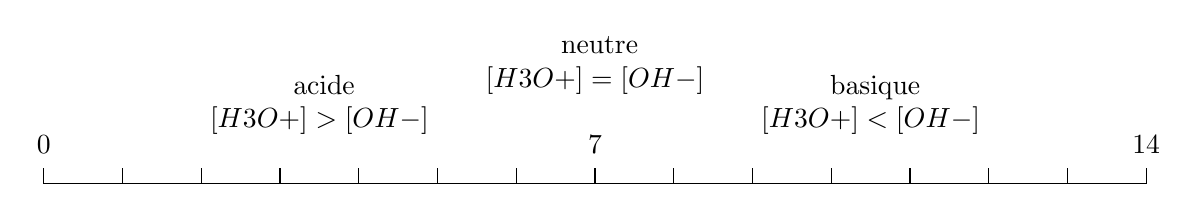
\begin{tikzpicture} \draw
        (0,0) -- (14,0);
        \foreach \i in {0,1,...,14} {
          \draw (\i,0) -- (\i,0.2);
        }
        \node at (0,0.5) {0};
        \node at (7,0.5) {7};
        \node at (14,0.5) {14};
      \node at (3.5,1) {\begin{minipage}{3cm}\begin{center}$\ph$ acide\\$[\ce{H3O+}] > [\ce{OH-}]$\end{center}\end{minipage}};
      \node at (7,1.5) {\begin{minipage}{3cm}\begin{center}$\ph$ neutre\\$[\ce{H3O+}] = [\ce{OH-}]$\end{center}\end{minipage}};
      \node at (10.5,1) {\begin{minipage}{3cm}\begin{center}$\ph$ basique\\$[\ce{H3O+}] < [\ce{OH-}]$\end{center}\end{minipage}};
      \end{tikzpicture}
    }
  \end{center}
  \caption{Échelle des $\ph$}
  \label{fig:ph_scale}
\end{figure}

Schéma général d'une réaction acide-base:
\[ \ce{Acide 1 + Base 2 <=> Base_{conj}1 + Acide_{conj}2} \]

$$\kc=\frac{K_{a1}}{K_{a2}}$$

\subsection{Prévoir le sens d'évolution des réactions acide-base}

\begin{itemize}
  \item[$\bullet$] Qualitativement: la réaction évolue préférentiellement dans le sens qui consomme l'acide et la base les plus forts et produits les plus faibles.
  \item[$\bullet$] Quantitativement:
    \begin{itemize}
      \item Si $\kc>10^3$: réaction complète
      \item Si $\kc<10^{-3}$: réaction impossible
      \item Si $10^{-3}<\kc<10^3$: réaction équilibrée avec une évolution
        préférentielle de la réaction de la gauche vers la droite si $\kc>1$.
    \end{itemize}
\end{itemize}

\subsection{$\ph$ des acides et des bases en solution aqueuse}

\subsubsection{Acide fort}
Un acide fort est un électrolyte fort $\rightarrow$ dissociation totale
en solution aqueuse.

\[ \ph = -\log{[\ce{H3O+}]} \]

\subsubsection{Base forte}
Une base forte est un électrolyte fort $\rightarrow$ dissociation toale
en solution aqueuse.

\[ \ph = -\log{[\ce{H3O+}]} = -\log{\frac{K_w}{[\ce{OH-}]}} = 14 + \log{[\ce{OH-}]} \]

\paragraph{Solution très diluée d'acide fort ou de base forte}
Dans les solutions d'acides ou de bases forts très diluées ($<\unit{10^{-6}}{\mole\per\liter}$),
le $\ph$ est influencé par l'autoprotolyse de l'eau de façon significative. Il faut alors procèder
en trois étapes\cite[p.~464]{atkins2011principes} :

\begin{enumerate}
	\item Ecriture de l'équation d'équilibre des charges ;
	\item Ecriture de l'équation de conservation de la matière ;
	\item Expression de la constante d'autoprotolyse.
\end{enumerate}

A partir des ces 3 équations, on peut obtenir une équation d'une deuxième
degré dont l'inconnue est [\ce{H3O+}].

\subsubsection{Acide faible}

\[ \ce{HA + H2O <=> H3O+ + A-} \]

Un acide faible est un électrolyte faible $\rightarrow$ dissociation
partielle en solution aqueuse. On définit le pourcentage de
déprotonation d'un acide faible :

\[ \text{\% de déprotonation} = \frac{[\ce{A-}]}{[\ce{HA}]_{\text{initiale}}} \cdot 100\]

Pour calculer la concentration en \ce{H3O+}, on écrit ensuite un tableau d'avancement :

\begin{table}[!ht]
	\centering
	\begin{tabular}{c|ccc}
								& \ce{HA} 					& \ce{H3O+} & \ce{A-} \\
		\hline
		$c_i$ 			& $[\ce{HA}]_i$ 		& 0					& 0 \\
		$\Delta c$	&	$-x$ 							& $+x$			& $+x$ \\
		$c_{eq}$		& $[\ce{HA}]_i - x$ & $x$				& $x$
	\end{tabular}
\end{table}

On peut alors écrire :

\[ K_a = \frac{x^2}{[\ce{HA}]_i -x} \]

et résoudre l'équation pour trouver $x$ : la concentration en \ce{H3O+}.

\subsubsection{Base faible}
\[ \ce{B + H2O <=> BH+ + OH-} \]

Une base faible est un électrolyte faible $\rightarrow$ dissociation
partielle en solution aqueuse. On définit le pourcentage de
déprotonation d'une base faible :

\[ \text{\% de déprotonation} = \frac{[\ce{BH+}]}{[\ce{B}]_{\text{initiale}}} \cdot 100\]

Pour calculer la concentration en \ce{OH-}, on écrit ensuite un tableau d'avancement :

\begin{table}[!ht]
	\centering
	\begin{tabular}{c|ccc}
								& \ce{B} 					& \ce{BH+} & \ce{OH-} \\
		\hline
		$c_i$ 			& $[\ce{B}]_i$ 		& 0					& 0 \\
		$\Delta c$	&	$-x$ 							& $+x$			& $+x$ \\
		$c_{eq}$		& $[\ce{B}]_i - x$ & $x$				& $x$
	\end{tabular}
\end{table}

On peut alors écrire :

\[ K_b = \frac{K_w}{K_{\text{acide conj.}}} = \frac{x^2}{[\ce{B}]_i -x} \]

et résoudre l'équation pour trouver $x$ : la concentration en \ce{OH-}. On retrouve
alors facilement la concentration en \ce{H3O+}.

\paragraph{Remarque}
Dans le cas d'un acide faible ou d'une base faible, si le \% de déprotonation est inférieur
à 5\%, on peut négliger le $-x$ au dénominateur de la constante d'acidité ou de basicité.

\subsection{$\ph$ des solutions de sel}

\begin{itemize}
	\item[$\bullet$] Sels acides: sels résultant de la réaction d'un acide fort avec une base faible (ex: \ce{HCl(aq) + NH+(aq) -> NH4Cl(aq)}).
    Comme le sel est un électrolyte fort,
    il se dissocie totalement dans la solution aqueuse (voir exemple~11.10, \cite[p.~452]{atkins2011principes}).
  \item[$\bullet$] Sels basiques: sels résultant de la réaction d'un acide faible et d'une base forte (ex: \ce{CH3COOH(aq) + NaOH(aq) -> CH3COONa(aq) + H2O(l)})
	(voir exemple~11.11, \cite[p.~453]{atkins2011principes})
  \item[$\bullet$] Sels neutres: sels résultant de la réaction d'un acide fort et d'une base forte.
    Ex: \ce{HCl(aq) + KOH(aq) -> KCl(aq) + H2O(l)}: ni \ce{K+} ni \ce{Cl-} ne réagissent avec l'eau car HCl (acide fort) et KOH (base forte) n'existent pas en solution aqueuse.
\end{itemize}

\section{Equilibre en phase aqueuse}
\subsection{Solutions tampons}
Une solution tampon est constituée à la fois d'un acide faible et de sa base conjuguée ou d'une base faible et de son acide conjugué.
\[ \ce{HA + H2O <=> A- + H3O+} \]

\subsubsection{$\ph$ des solutions tampons}
Les tampons stabilisent le $\ph$ d'une solution en fournissant une source ou un piège à protons.

$$\ph = \pka + \log{\frac{{[\ce{A-}]_i}}{{[\ce{HA}]_i}}}$$

On observe donc que le $\ph$ d'une solution tampon $\approx \pka$ si $[\ce{A-}]_i \approx [\ce{HA}]_i$.
Le choix du tampon doit être fait de manière telle que :

\[ \pka \approx \ph \text{ recherché} \]

Pour $0.1 < \frac{{[\ce{A-}]_i}}{{[\ce{HA}]_i}} < 10$, la zone tampon est donc $\pka \pm 1$.

\paragraph{Remarque}
Si un sel est formé, il faut tenir compte de son caractère acide ou basique.

\subsubsection{Pouvoir tampon}
On définit le pouvoir tampon :

\[ \text{Pouvoir tampon} = \frac{\Delta n}{\Delta\ph} \]

Où $n$ est le nombre de millimole de base ou d'acide ajouté.

% Revoir la forme de ce résumé (sous-forme de schéma?)
\subsection{Résumé}
Acide Fort +
\begin{itemize}
  \item[$\bullet$] Base Forte:
    \begin{itemize}
      \item si excès d'acide $\rightarrow$ AF
      \item si équivalence $\rightarrow$ sel neutre
      \item si excès de base $\rightarrow$ BF
    \end{itemize}
  \item[$\bullet$] acide faible $\rightarrow$ A.F. dilué
  \item[$\bullet$] base faible:
    \begin{itemize}
      \item si excès d'AF $\rightarrow$ AF dilué
      \item si équivalence $\rightarrow$ sel acide
      \item si excès bf $\rightarrow$ mélange tampon
    \end{itemize}
  \item[$\bullet$] sel acide $\rightarrow$ AF dilué
  \item[$\bullet$] sel neutre $\rightarrow$ AF dilué
  \item[$\bullet$] sel basique:
    \begin{itemize}
      \item si excès sel $\rightarrow$ mélange tampon
      \item si équivalence $\rightarrow$ af
      \item si excès AF $\rightarrow$ AF dilué
    \end{itemize}
  \item[$\bullet$] mélange tampon bf et son sel:
    \begin{itemize}
      \item si excès AF $\rightarrow$ AF dilué
      \item si équivalence $\rightarrow$ sel acide
      \item si excès bf $\rightarrow$ mélange tampon
    \end{itemize}
  \item[$\bullet$] tampon af et son sel
    \begin{itemize}
      \item si excès AF $\rightarrow$ AF dilué
      \item si équivalence $\rightarrow$ af
      \item si excès af $\rightarrow$ mélange tampon
    \end{itemize}
\end{itemize}
(Même principe pour les Bases Fortes)

acide faible +
\begin{itemize}
  \item[$\bullet$] sel neutre $\rightarrow$ af dilué
  \item[$\bullet$] sel basique de l'af et BF $\rightarrow$ mélange tampon
\end{itemize}

base faible + sel acide de la bf et AF $\rightarrow$ mélange tampon

\section{Titrages acido-basiques}
Un titrage permet de déterminer les concentrations d'une solution inconnue à partir d'une solution de concentration connue.

Le point d'équivalence est le moment où :

$$N_BV_B = N_AV_A \Leftrightarrow n_{\ce{OH-}} = n_{\ce{H3O+}}$$ (mais $\ph\neq 7$ \emph{sauf si} acide fort et base forte).
Pour le détecter $\rightarrow$ indicateur coloré (acide faible) qui change de couleur selon sa forme ionisée. Le changement
de couleur se produit lorsque $\ph = {\pka}_{\text{indicateur}}$.

Une courbe de titrage (ou courbe de $\ph$) est le graphique de l'évolution du $\ph$ de la solution
à tritrer en fonction du volume de la solution titrante ajoutée au cours du titrage \cite[p.~484-490]{atkins2011principes}.

\subsection{Titrage acide fort/base forte (et inversement)}
Pour calculer le $\ph$ au cours d'un titrage acide fort/base forte (ou inversement) :

\begin{enumerate}
	\item Calculez la quantité d’ions \ce{H3O+} (si la solution à titrer est un acide fort) ou
				la quantité d’ions \ce{OH-} (si la solution à titrer est une base forte) ;
	\item Calculez la quantité d’ions ce{OH-} (si le réactif de titrage est une base forte)
				ou d’ions \ce{H3O+} (si le réactif de titrage est un acide fort) ;
	\item	Ecrivez l’équation chimique équilibrée de la réaction de neutralisation et
				calculez la quantité d’ions \ce{H3O+} (ou d’ions \ce{OH-} , si la solution à titrer est
				une base forte) restante dans la solution après réaction avec tout le
				réactif de titrage ajouté ;
	\item Calculez le $\ph$.
\end{enumerate}

\subsection{Titrage acide faible/base forte (et inversement)}
Le $\ph$ est régi par le soluté présent majoritairement dans la solution. Comme pour les solutions
tampons, il faut tenir compte de l'influence du sel sur le $\ph$.

\paragraph{Remarque}
Le $\ph$ au demi-point d'équivalence est égal au $\pka$ de l'acide (figure~12.8, \cite[p.~490]{atkins2011principes}).

\subsection{Neutralisation d'un acide fort (HCl) par une base forte (NaOH)}
La neutralisation se fait selon le diagramme bilan figurant sur la Figure~\ref{fig:diagbil}.

\begin{figure}[ht!]
  \begin{center}
    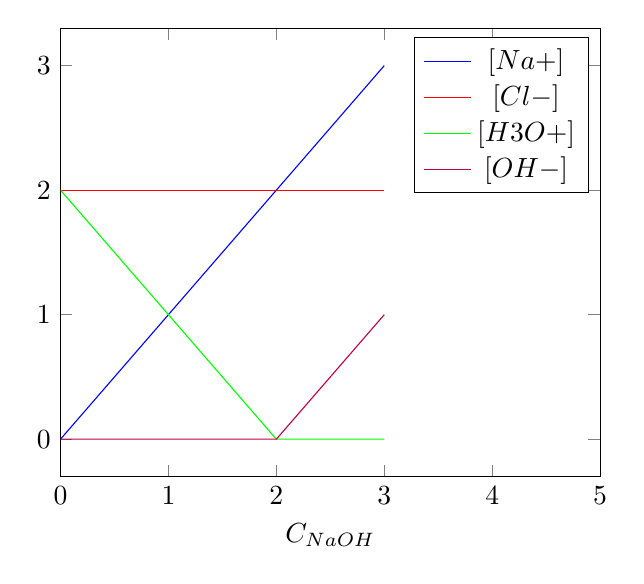
\begin{tikzpicture}
      \begin{axis}[xlabel=$C_{\ce{NaOH}}$,
        xmin=0,xmax=5]
        \addplot[color=blue] coordinates{(0,0)(2,2)(3,3)};
        \addlegendentry{$[\ce{Na+}]$}
        \addplot[color=red] coordinates{(0,2)(2,2)(3,2)};
        \addlegendentry{$[\ce{Cl-}]$}
        \addplot[color=green] coordinates{(0,2)(2,0)(3,0)};
        \addlegendentry{$[\ce{H3O+}]$}
        \addplot[color=purple] coordinates{(0,0)(2,0)(3,1)};
        \addlegendentry{$[\ce{OH-}]$}
      \end{axis}
    \end{tikzpicture}
  \end{center}
  \caption{Diagramme bilan}
  \label{fig:diagbil}
\end{figure}

\subsection{Equilibres de solubilité}
\subsubsection{Solution, soluté et solubilté}
Une \textbf{solution} est une phase liquide homogène qui consiste en un mélange homogène
de plusieurs substances en proportions variables.

Le \textbf{solvant} désigne le composant en excès (le plus souvent il s'agit de l'eau).
Les \textbf{solutés} désignent les composants minoritaires (composés ioniques, sels).

Une solution est dite \textbf{saturée} lorsque l'on a atteint la quantité maximale que l'on peut
dissoudre dans le solvant.

La \textbf{solubilité}, notée $s$, est la quantité maximale de soluté dissoute à une température
donnée dans un litre de solution saturée. Elle s'exprime en  $\gram\per\liter$ ou en $\mole\per\liter$.

Par convention :

\begin{itemize}
	\item Soluble si $s \geq \unit{0.1}{\mole\per\liter}$ ;
	\item Insoluble si $s \leq \unit{0.001}{\mole\per\liter}$.
\end{itemize}

\subsubsection{Produit de solubilité}

\[ \ce{M_nN_m(s) <=> mM^{n+}(aq) + nN^{m-}(aq)} \]

La constante d'équilibre de cette réaction est appelée le produit de solubilité et
est donné par :

\[ K_s = [\ce{M^{n+}}]^m [\ce{N^{m-}}]^n \]

En écrivant le tableau d'avancement de la réaction en fonction de la solubilité $s$ :

\begin{table}[!ht]
	\centering
	\begin{tabular}{c|ccc}
								& \ce{M_nN_m(s)} 	& \ce{mM^{n+}} 	& \ce{nN^{m-}} \\
		\hline
		$c_i$ 			& $c_i$ 					& 0							& 0 \\
		$c$					& $c_i - s$ 			& $ms$					& $ns$
	\end{tabular}
\end{table}

on trouve que :

\[ K_s = (ms)^m(ns)^n \]

\subsubsection{Effet de l'ion commun}
L'effet d'ion commun est la diminution de la solubilité d'un sel peu soluble
par l'addition d'un sel soluble qui a un ion commun avec lui.

\paragraph{Exemple}
On cherche à calculer la solubilité molaire du \ce{PBCl_2(s)} dans \ce{CaCl_2(aq)} $\unit{0,025}{\mole\per\liter}$.
On remarque un ion commun entre le soluté et le solvant. Dressons un tableau d'avancement de la réaction :

\begin{table}[!ht]
	\centering
	\begin{tabular}{c|ccc}
								& \ce{PbCl_2(s)} 	& \ce{Pb^{2+}(aq)} 	& \ce{2Cl^-(aq)} \\
		\hline
		$c_i$ 			& $c_0$ 					& 0								& $2 \cdot 0,025$ \\
		$c$					& $c_0 - s$ 			& $s$							& $0,050 +2s$
	\end{tabular}
\end{table}

On va supposer ici que la quantité d'ions chlorure apporté par la dissolution du \ce{PbCl2(s)}
est largement inférieure à la quantité d'ions chlorure dans la solution de \ce{CaCl2(aq)} :
$2s \ll 0.050$. Le $K_s$ du \ce{PbCl2(s)} vaut $1,6 \cdot 10^{-5}$ et on trouve alors
$s = \unit{6,4 \cdot 10^{-3}}{\mole\per\liter}$.

\subsubsection{Réactions de précipitation}
Une réaction de \textbf{précipitation} se produit lorsque deux solutions
d'électrolytes forts se mélangent et réagissent pour donner un solide insoluble.

\paragraph{Prédire la précipitation}
\begin{itemize}
	\item	Si $Q_r < K_s$ : dissolution ;
	\item Si $Q_r > K_s$ : précipitation.
\end{itemize}

\paragraph{Exemple}
On cherche à savoir si un précipité de \ce{Ag2CO3} va se former si on mélange
\unit{5}{\milli\liter} de \ce{K2CO3(aq)} \unit{0,10}{\mole\per\liter} et \unit{1}{\liter}
de \ce{AgNo3(aq)} \unit{0.01}{\mole\per\liter}.

On commence par écrire la réaction (débarassée des ions spectateurs) :

$$\ce{Ag2CO3(s) -> CO3(aq) + 2Ag(aq}$$

On calcule ensuite $Q_s = [\ce{CO3}][\ce{Ag}]^2 = 4,925 \cdot 10^{-8}$ que l'on compare
à la valeur (prise dans une table) de $K_s = 6,2 \cdot 10^{-12}$.
Comme $Q_s > K_s$, il y aura précipitation.

\paragraph{Précipitation sélective}
On peut séparer un mélange d'ions en solution en ajoutant un ion
de charge opposée avec lequel ils forment des sels ayant des solubilités
différentes.

Voir exemple~12.11, \cite[p.~503]{atkins2011principes}.

\subsubsection{Réaction de dissolution des précipités}
On peut augmenter la solubilité d'un solide en éliminant l'un de ses ions
de la solution.

\paragraph{Dissolution par réaction de l'anion}
On peut utiliser un acide pour dissoudre un précipité contenant
des ions hydroxydes, sulfure, sulfite ou carbonate.

\paragraph{Dissolution par réaction du cation (réactions de complexation)}
La solubilité d'un sel augmente si le sel peut former un ion
complexe avec une autre espère en solution.

\paragraph{Exemple}
On cherche à calculer la solubilité du \ce{AgBr(s)} dans \ce{NH3(aq)} en
sachant que le bromure d'argent dans l'ammoniac forme du \ce{Ag(NH3)2+}.
On écrit d'abord la réaction de dissolution de constante $K_s$

$$\ce{AgBr(s) <=> Ag+(aq) + Br-(aq)}$$

et l'équation de formation de l'ion complexe (disponible dans une table)
de constante de formation $K_f$

$$\ce{Ag+(aq) + 2NH3(aq) <=> Ag(NH3)2+(aq)}$$

On somme ensuite ces deux réactions pour obtenir la réaction globale

$$\ce{AgBr(s) + 2NH3(aq) <=> Ag(NH3)2+(aq) + Br-(aq)}$$

de constante $K = K_f \cdot K_s = \frac{[Ag(NH3)2+)][Br-]}{[NH3]^2}$.

On calcule alors un tableau d'avancement :

\begin{table}[!ht]
	\centering
	\begin{tabular}{c|ccc}
								& \ce{2NH3(aq)} 	& \ce{Ag(NH3)2+} 	& \ce{Br-} \\
		\hline
		$c_i$ 			& $1$							& 0								& 0 \\
		$c$					& $1-2x$ 					& $x$							& $x$
	\end{tabular}
\end{table}

Et il ne reste plus qu'à déterminer $[\ce{Br-}] = x$ en utilisant $K$.

\annexe
\section{Notations}
\label{ann:nota}
De nombreuses notations seront utilisées au cours de cette synthèse.
Pour des raisons de concision,
leur signification ne sera pas rappelée à chaque fois mais elle sera indiqué dans la Table~\ref{tab:notations}.
\begin{table}[h!]
  \begin{center}
    \begin{tabular}{ll}
      $\nu$ & La fréquence d'un rayonnement électromagnétique\\
      $\lambda$ & La longeur d'onde d'un rayonnement électromagnétique\\
      $c$ & La vitesse d'un rayonnement électromagnétique\\
      $c_0$ & La vitesse de la lumière dans le vide\\
      $p$ & Quantité de mouvement d'un corps\\
      $h$ & La constante de Planck\\
      $E_A$ & \'Electroaffinité d'un atome,
      voir section~\ref{sec:electro} page~\pageref{sec:electro}\\
      $E_I$ & \'Energie d'ionisation d'un atome,
      voir section~\ref{sec:ioni} page~\pageref{sec:ioni}\\
      $E_N$ & \'Energie de neutralisation entre deux atomes (liaison ionique),
      voir section~\ref{sec:neutral} page~\pageref{sec:neutral}\\
      $E_l$ & \'Energie de liaison covalente,
      voir section~\ref{sec:E_l} page~\pageref{sec:E_l}\\ % FIXME: E_l ou E_D ?
      $N_A$ & Nombre d'avogadro\\
      %$r$ & Le rayon d'un atome\\
      $C_s$ & Capacité calorifique spécifique d'un corps,
      voir section~\ref{sec:C_s} page~\pageref{sec:C_s}\\
      $\ccal$ & Capacité calorifique d'un corps,
      voir section~\ref{sec:C_cal} page~\pageref{sec:C_cal}\\
      $\Delta H$ & Variation d'enthalpie,
      voir section~\ref{sec:DH} page~\pageref{sec:DH}
    \end{tabular}
    \caption{Répertoire des notations}
    \label{tab:notations}
  \end{center}
\end{table}

\section{Différentes énergies}

Quand on travail avec des énergies,
il faut faire bien attention de les utiliser dans le bon sens.
Est-ce l'énergie à fournir au système,
c'est à dire absorbée par le système ou dégagée par le système ?
La Table~\ref{tab:energies} essaie de rassembler toutes ces conventions.

\begin{table}[h!]
  \begin{center}
    \begin{tabular}{|p{0.1\textwidth}|p{0.35\textwidth}|p{0.35\textwidth}|p{0.2\textwidth}|}
      \hline
      Symbole & Description & Valeur (par rapport au système) & Référence\\
      \hline
      $E_A$ & \'Electroaffinité d'un atome & Dégagée pour capter un $e^-$ & \ref{sec:electro} p.~\pageref{sec:electro}\\
      $E_I$ & \'Energie d'ionisation d'un atome & Absorbée pour relacher un $e^-$ & \ref{sec:ioni} p.~\pageref{sec:ioni}\\
      $E_N$ & \'Energie de neutralisation & Aborbée pour lier deux atomes déjà ionisés & \ref{sec:neutral} p.~\pageref{sec:neutral}\\
      $E_l$ & \'Energie de liaison & Absorbée pour casser la liaison & \ref{sec:E_l} p.~\pageref{sec:E_l}\\ % FIXME: E_l ou E_D ?
      \hline
    \end{tabular}
    \caption{Répertoire des énergies}
    \label{tab:energies}
  \end{center}
\end{table}

\section{De réactifs et produits à réaction}
Souvent,
on sait calculer les données pour les produits et
les réactifs mais on aimera les avoir pour la réaction.
Voilà comment passer de l'un à l'autre,
avec $v_p$ les coefficients des produits et
$v_r$ les coefficients des réactifs,
\begin{align*}
  \Delta S\std &= \sum v_p S\std_\mathrm{produits}
  - \sum v_r S\std_\mathrm{réactifs}\\
  \Delta H &= \sum v_p \Delta {H_f}_\mathrm{produits}
  - \sum v_r \Delta {H_f}_\mathrm{réactifs}
\end{align*}
Si des molécules sont déjà dans les états voulus,
on a juste
\[ \Delta H = \sum v_r{E_l}_\mathrm{réactifs} - \sum v_p{E_l}_\mathrm{produits} \]

\section{Schéma de synthèse sur les liaisons chimiques}
\label{sec:synthese_liaisons}

\begin{center}
  \scalebox{0.98}{\rotatebox{90}
    {\Tree [.{Liaisons chimiques} [.{Intramoléculaires \\ $E_L > \numprint[\kilo\joule\per\mole]{40}$}
          Métalliques [.{Covalentes \\ $\Delta \chi < 1,5$} {Pures \\ $\Delta \chi = 0$} Polarisées
        Datives ] {Ioniques \\ $\Delta \chi > 2$} ] [.{Intermoléculaires \\ $E_L < \numprint[\kilo\joule\per\mole]{40}$}
          [.{Van der Waals} {Keesom \\ Permanent-permanent} {Debye \\ Permanent-induit} {London \\ Induit-induit} ]
  {Ponts H \\ \ce{H} et \ce{F}, \ce{O}, \ce{N}} ] ]}}
\end{center}

\biblio
\end{document}
